


\documentclass[10.5pt]{article}

\usepackage[top=.8in, bottom=.6in, left=.56in, right=.45in, 
paperheight=13.25in,paperwidth=9.25in]{geometry}


\usepackage{setspace}

\newcommand{\Ldown}[1]{\hspace{-2pt}\raisebox{-1pt}{{%\fontfamily{lmhh}
\fontsize{14}{11}\selectfont{}{\textnormal{#1.}}}}\hspace{3pt}}


\newcommand{\semihr}[1]{{\textcolor{orange!60!black}{\hrule width #1}}}


\usepackage{xcolor}


\usepackage{xcolor}



%\input{commands}

\newcommand{\mdash}{---}
\newcommand{\q}[1]{``#1''}
\newcommand{\br}{

}

\newcommand{\raggedRightTitle}[1]{\br{}\begin{flushleft}\textbf{#1}\end{flushleft}}

%\newcommand{\visavis}{vis-\`a-vis}


%\input{ngml/ngml-setup-commands}
%\input{ngml/ngml-sdi-commands}
%\input{ngml/ngml-deco-commands}

%\AtEndDocument{\immediate\write18{cd /home/nlevisrael/gits/ntxh/wip-sebi/ar/code/cpp/qmake-console/projects/gtagml/ngml-sdi-console; ./run-with-args.sh /home/nlevisrael/gits/ntxh/wip-sebi/gtagml/ctg/gen/ctg/ctg.gt.tex /home/nlevisrael/gits/ntxh/wip-sebi/gtagml/ctg/gen/ctg/ctg.gt.sdi.ntxh /home/nlevisrael/gits/ntxh/wip-sebi/gtagml/ctg/gen/ctg/ctg.gt.sdi-prelatex.ntxh; cd -;}}



% pmml  arff  openannotation

\usepackage[T1]{fontenc}
\usepackage{tgtermes}

\usepackage[hang,flushmargin]{footmisc}

\usepackage{titlesec}

\titlespacing*{\section}
{0pt}{4ex plus 1ex minus .5ex}{.1ex plus .2ex}

%\usepackage{titlesec}

\titleformat{\section}
  {\normalfont\Large\bfseries}   % The style of the section title
  {}                             % a prefix
  {0pt}                          % How much space exists between the prefix and the title
  {} 


%\usepackage{mathptmx}

\usepackage{eso-pic}

\AddToShipoutPictureBG{%

\colorlet{redbl}{red!40!magenta}
\colorlet{yelbl}{yellow!60!magenta}

\colorlet{redblg}{redbl!30!black}

\ifnum\value{page}>66{
\AtTextLowerLeft{\raisebox{-21pt}{\hspace{-15pt}\fontfamily{qtm}\fontsize{10}{11}\fontseries{b}\selectfont{}{\colorbox{yelbl!7}{\textcolor{redblg!70}{PLEASE SEE OUR SOFTWARE DEMO VIDEOS: \href{http://www.lingtechsys.com/videos/qmt-composite.mkv}{GIS},
\href{http://www.lingtechsys.com/videos/dhax-composite.mkv}{360\textdegree{} photography}, and \href{http://www.lingtechsys.com/videos/xcsd-composite.mkv}{image processing}.}}}}}
}\fi
}


%\setlength\parindent{0pt}

\AddToShipoutPictureBG{%

\ifnum\value{page}>1{
\AtTextUpperLeft{
\makebox[18.5cm][r]{
\raisebox{-1.63cm}{%
{\transparent{0.3}{\includegraphics[width=0.29\textwidth]{e-logo.png}}	}} } }
}\fi
}

\AddToShipoutPicture{%
{
 {\color{blGreen!70!red}\transparent{0.9}{\put(0,0){\rule{3pt}{\paperheight}}}}%
 {\color{darkRed!70!purple}\transparent{1}\put(3,0){{\rule{4pt}{\paperheight}}}}
% {\color{logoPeach!80!cyan}\transparent{0.5}{\put(0,700){\rule{1cm}{.6cm}}}}%
% {\color{darkRed!60!cyan}\transparent{0.7}\put(0,706){{\rule{1cm}{.6cm}}}}
% \put(18,726){\thepage}
% \transparent{0.8}
}
}

%\AddToShipoutPicture{%
%\ifnum\value{page}=1
%\put(247.5,988){%
%	\transparent{0.7}{
%		\includegraphics[width=0.4\textwidth]{logo.png}}}
%\fi
%}	


\AddToShipoutPictureBG{%
\ifnum\value{page}=14

\put(7,678){
	\transparent{1}{
		\includegraphics[angle=0.5,origin=c,width=0.4\textwidth]{pm/1a.jpg}}}


\put(241,698){
	\transparent{1}{
		\includegraphics[angle=0,origin=c,width=0.31\textwidth,
trim=0 14mm 0 10mm, clip]{pm/7a.png}}}


\put(6,492){
	\transparent{1}{
		\includegraphics[angle=-0.5,origin=c,width=0.4\textwidth]{pm/5a.png}}}


\put(452,712){
	\transparent{1}{
		\includegraphics[angle=-1,origin=c,width=0.3\textwidth]{pm/2a.png}}}



\put(442,681){
	\transparent{1}{
		\includegraphics[angle=0,origin=c,width=0.18\textwidth]{pm/8a.png}}}


%\put(412,680){
%	\transparent{1}{
%		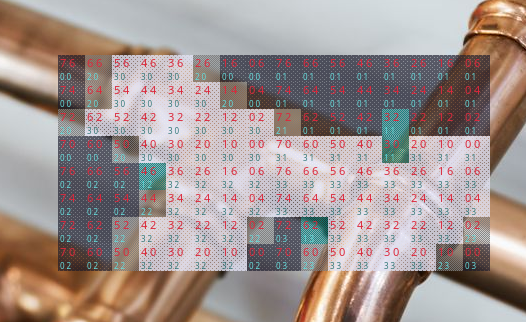
\includegraphics[angle=2.5,origin=c,width=0.2\textwidth]{pm/8.png}}}


\put(402,487){
	\transparent{1}{
		\includegraphics[angle=-1,origin=c,width=0.45\textwidth]{pm/3a.jpg}}}

\fi
}	




%\pagestyle{empty} % no page number
%\parskip 7.2pt    % space between paragraphs
%\parindent 12pt   % indent for new paragraph
%\textwidth 4.5in  % width of text
%\columnsep 0.8in  % separation between columns

%\setlength{\footskip}{-3pt}

%\usepackage[paperheight=15in,paperwidth=8.5in]{geometry}
%\geometry{left=.65in,top=.65in,right=.45in,bottom=1.25in} %margins

%\renewcommand{\thepage}{\raisebox{2pt}{\arabic{page}}}

\renewcommand{\footnoterule}{%
	\kern -3pt
	\hrule width .92\textwidth height .5pt
	\kern 10pt
}


\usepackage[hyphens]{url}
\newcommand{\biburl}[1]{ {\fontfamily{gar}\selectfont{\textcolor[rgb]{.2,.6,0}%
{\scriptsize {\url{#1}}}}}}

%\linespread{1.3}

\newcommand{\sectsp}{\vspace{12pt}}

\usepackage{graphicx}
\usepackage{color,framed}

\usepackage{textcomp}

\usepackage{float}

\usepackage{mdframed}


\usepackage{setspace}

\usepackage{xcolor}

\usepackage[hyphenbreaks]{breakurl}
\usepackage[hyphens]{url}

\usepackage{hyperref}

\colorlet{blCyan}{cyan!50!blue}

\definecolor{darkRed}{rgb}{.2,.0,.1}


\definecolor{blGreen}{rgb}{.2,.7,.3}

\definecolor{darkBlGreen}{rgb}{.1,.3,.2}

\definecolor{oldBlColor}{rgb}{.2,.7,.3}

\definecolor{blColor}{rgb}{.1,.3,.2}

\definecolor{elColor}{rgb}{.2,.1,0}
\definecolor{flColor}{rgb}{0.7,0.3,0.3}

\definecolor{logoOrange}{RGB}{108, 18, 30}
\definecolor{logoGreen}{RGB}{85, 153, 89}
\definecolor{logoPurple}{RGB}{200, 208, 30}

\definecolor{logoBlue}{RGB}{4, 2, 25}
\definecolor{logoPeach}{RGB}{255, 159, 102}
\definecolor{logoCyan}{RGB}{66, 206, 244}
\definecolor{logoRed}{rgb}{.3,0,0}

\newcommand{\colorq}[1]{{\color{logoOrange!70!black}{\q{\small\textbf{#1}}}}}

\let\qq\q

\definecolor{inOne}{rgb}{0.122, 0.435, 0.698}% Rule colour
\definecolor{inTwo}{rgb}{0.122, 0.698, 0.435}% Rule colour

\definecolor{outOne}{rgb}{0.435, 0.698, 0.122}% Rule colour
\definecolor{outTwo}{rgb}{0.698, 0.435, 0.122}% Rule colour

\colorlet{linkcolor}{flColor!60!red}


\hypersetup{
	colorlinks=true,
	citecolor=blCyan!40!green,
	filecolor=magenta!30!logoBlue,
	urlcolor=blue,
    linkcolor=linkcolor!70!black,
%    allcolors=blCyan!40!green
}


\usepackage[many]{tcolorbox}% http://ctan.org/pkg/tcolorbox

\usepackage{transparent}

\newlength{\bsep}
\setlength{\bsep}{-1pt}
\let\xbibitem\bibitem
\renewcommand{\bibitem}[2]{\vspace{\bsep}\xbibitem{#1}{#2}}

\newenvironment{cframed}{\begin{mdframed}[linecolor=logoPeach,linewidth=0.4mm]}{\end{mdframed}}

\newenvironment{ccframed}{\begin{mdframed}[backgroundcolor=logoGreen!5,linecolor=logoCyan!50!black,linewidth=0.4mm]}{\end{mdframed}}

\usepackage{aurical}
\usepackage[T1]{fontenc}

\usepackage{relsize}

\newcommand{\bref}[1]{\hspace*{1pt}\textbf{\ref{#1}}}

\newcommand{\dashsep}{--\hspace*{5pt}}

\newcommand{\pseudoIndent}{

\vspace{2pt}\hspace*{6pt}}

\usepackage{titlesec}

\titlespacing*{\subsection}
{0pt}{5ex plus 1ex minus .2ex}{0.5ex plus .2ex}


%\titlespacing*{\section}
%{0pt}{3.5ex plus 1ex minus .2ex}{1ex plus .2ex}

%
\newcommand{\deconum}[1]{{\protect\raisebox{-1pt}{{\LARGE #1}}}}

\newcommand{\visavis}{vis-\`a-vis}

\newcommand{\VersatileUX}{{\color{red!85!black}{\Fontauri Versatile}}%
{{\fontfamily{qhv}\selectfont\smaller UX}}}

\newcommand{\NDPCloud}{{\color{red!15!black}%
{\fontfamily{qhv}\selectfont {\smaller NDP C{\smaller LOUD}}}}}

\newcommand{\MThreeK}{{\color{blGreen!45!black}%
{\fontfamily{qhv}\fontsize{10}{8}\selectfont {M3K}}}}


\newcommand{\lfNDPCloud}{{\color{red!15!black}%
{\fontfamily{qhv}\selectfont N{\smaller DP C{\smaller LOUD}}}}}

\newcommand{\textds}[1]{{\fontfamily{lmdh}\selectfont{%
\raisebox{-1pt}{#1}}}}

\newcommand{\dsC}{{\textds{ds}{\fontfamily{qhv}\selectfont \raisebox{-1pt}
{\color{red!15!black}{C}}}}}

\definecolor{tcolor}{RGB}{24,52,61}

\newcommand{\CCpp}{\resizebox{!}{7pt}{\AcronymText{C}}/\Cpp{}}
\newcommand{\NoSQL}{\resizebox{!}{6pt}{\AcronymText{NoSQL}}}
\newcommand{\SQL}{\resizebox{!}{7pt}{\AcronymText{SQL}}}

\newcommand{\NCBI}{\resizebox{!}{7pt}{\AcronymText{NCBI}}}
\newcommand{\BioNetGen}{\resizebox{!}{7pt}{\AcronymText{BioNetGen}}}
\newcommand{\BNGL}{\resizebox{!}{7pt}{\AcronymText{BNGL}}}

\newcommand{\GML}{\resizebox{!}{7pt}{\AcronymText{GML}}}

\newcommand{\GIS}{\resizebox{!}{6pt}{\AcronymText{GIS}}}
\newcommand{\ACRIS}{\resizebox{!}{6pt}{\AcronymText{ACRIS}}}
\newcommand{\HPD}{\resizebox{!}{6pt}{\AcronymText{HPD}}}


\newcommand{\HTXN}{\resizebox{!}{7pt}{\AcronymText{HTXN}}}

\newcommand{\TDM}{\resizebox{!}{7pt}{\AcronymText{TDM}}}

\newcommand{\lHTXN}{\resizebox{!}{7.5pt}{\AcronymText{H}}%
\resizebox{!}{6pt}{\AcronymText{TXN}}}

\newcommand{\lsHTXN}{\resizebox{!}{9.5pt}{\AcronymText{\textcolor{tcolor}{HTXN}}}}

\newcommand{\LAF}{\resizebox{!}{7pt}{\AcronymText{LAF}}}

\newcommand{\UDpipe}{\resizebox{!}{7pt}{\AcronymText{UDpipe}}}

\newcommand{\C}{\resizebox{!}{7pt}{\AcronymText{C}}}

\newcommand{\TME}{\resizebox{!}{7pt}{\AcronymText{TME}}}

\newcommand{\TwoD}{\resizebox{!}{6pt}{\AcronymText{2D}}}




\usepackage{mdframed}

\newcommand{\cframedboxpanda}[1]{\begin{mdframed}[linecolor=yellow!70!blue,linewidth=0.4mm]#1\end{mdframed}}





\newcommand{\libSBML}{\resizebox{!}{7pt}{\AcronymText{libSBML}}}


\newcommand{\PVD}{\resizebox{!}{7pt}{\AcronymText{PVD}}}


\newcommand{\SDK}{\resizebox{!}{7pt}{\AcronymText{SDK}}}
\newcommand{\NLP}{\resizebox{!}{7pt}{\AcronymText{NLP}}}


\newcommand{\PDF}{\resizebox{!}{6pt}{\AcronymText{PDF}}}
\newcommand{\TEI}{\resizebox{!}{7.5pt}{\AcronymText{TE{\hspace*{.5pt}I}}}}
\newcommand{\SSML}{\resizebox{!}{7.5pt}{\AcronymText{SSML}}}
\newcommand{\ToBI}{\resizebox{!}{7.5pt}{\AcronymText{ToBI}}}

\newcommand{\MMBioS}{\resizebox{!}{6pt}{\AcronymText{MMBioS}}}

\newcommand{\VTK}{\resizebox{!}{6pt}{\AcronymText{VTK}}}


\newcommand{\AXF}{\resizebox{!}{7pt}{\AcronymText{AXF}}}

\newcommand{\HyperGraphDB}{\resizebox{!}{7pt}{\AcronymText{HyperGraphDB}}}


\newcommand{\lAXF}{\resizebox{!}{7.5pt}{\AcronymText{A}}%
\resizebox{!}{6pt}{\AcronymText{XF}}}


\newcommand{\lsAXF}{\resizebox{!}{8.5pt}{\AcronymText{AXF}}}

\newcommand{\AXFD}{\resizebox{!}{7pt}{\AcronymText{AXFD}}}

\newcommand{\lAXFD}{\resizebox{!}{7.5pt}{\AcronymText{A}}%
\resizebox{!}{6pt}{\AcronymText{XFD}}}


\newcommand{\IJST}{\resizebox{!}{7pt}{\AcronymText{IJST}}}

\newcommand{\BioC}{\resizebox{!}{7pt}{\AcronymText{BioC}}}

\newcommand{\CoNLL}{\resizebox{!}{7pt}{\AcronymText{CoNLL}}}
\newcommand{\CoNLLU}{\resizebox{!}{7pt}{\AcronymText{CoNLL-U}}}


\newcommand{\ePub}{\resizebox{!}{7pt}{\AcronymText{ePub}}}

%\lsLPF

\definecolor{atcColor}{RGB}{96, 17, 12}
%\textcolor{tcolor}{

\newcommand{\ATextCClr}[1]{\textcolor{atcColor}{\textbf{#1}}}

\newcommand{\ATexttclr}[1]{\textcolor{tcolor}{\textbf{#1}}}
\newcommand{\THQL}{\resizebox{!}{6pt}{\ATexttclr{THQL}}}


\newcommand{\ATextbk}[1]{\textcolor{black!50!cyan}{\textbf{#1}}}


%\newcommand{\lDHOS}{\resizebox{!}{7pt}{\ATexttclr{D}}%
%resizebox{!}{6pt}{\ATexttclr{HOS}}}

\newcommand{\PGVM}{\resizebox{!}{6pt}{\ATexttclr{PGVM}}}
\newcommand{\lPGVM}{\resizebox{!}{7pt}{\ATexttclr{PGVM}}}

\newcommand{\DHOS}{\resizebox{!}{6pt}{\ATexttclr{DHOS}}}
\newcommand{\lDHOS}{\resizebox{!}{7.5pt}{\ATexttclr{D}}\resizebox{!}{6pt}{\ATexttclr{HOS}}}
\newcommand{\sDHOS}{\resizebox{!}{6pt}{\ATexttclr{DHOS}}}

\newcommand{\sQt}{\resizebox{!}{6pt}{\ATexttclr{Qt}}}

\newcommand{\sPhVM}{\resizebox{!}{6pt}{\ATexttclr{P\hspace{.5pt}\textit{h}\hspace*{-.5pt}VM}}}


\newcommand{\PhVM}{\resizebox{!}{6pt}{\ATexttclr{P\hspace{.5pt}\textit{h}\hspace*{-.5pt}VM}}}
\newcommand{\lPhVM}{\resizebox{!}{7.5pt}{\ATexttclr{P}}\resizebox{!}{6pt}{\ATexttclr{\hspace{1pt}\textit{h}\hspace*{-.5pt}VM}}}


\newcommand{\MOC}{\resizebox{!}{7pt}{\AcronymText{MOC}}}
\newcommand{\SPARQL}{\resizebox{!}{7pt}{\AcronymText{SPARQL}}}
\newcommand{\GraphQL}{\resizebox{!}{7pt}{\AcronymText{GraphQL}}}

%{}, \QML{}, \GraphQL

\newcommand{\CCi}{\resizebox{!}{6pt}{\ATexttclr{CCi}}}
\newcommand{\XCSD}{\resizebox{!}{6pt}{\ATexttclr{XCSD}}}

\newcommand{\lXCSD}{\resizebox{!}{7pt}{\ATexttclr{XCSD}}}
\newcommand{\lCCi}{\resizebox{!}{7pt}{\ATexttclr{CCi}}}

%\newcommand{\ConceptsDB}{\resizebox{!}{6pt}{\ATexttclr{ConceptsDB}}}
%\newcommand{\lConceptsDB}{\resizebox{!}{7pt}{\ATexttclr{C}}\resizebox{!}{6pt}%{\ATexttclr{onceptsDB}}}


\newcommand{\GIT}{\resizebox{!}{7pt}{\AcronymText{GIT}}}

\newcommand{\LPF}{\resizebox{!}{7pt}{\AcronymText{LPF}}}
\newcommand{\lLPF}{\resizebox{!}{8.5pt}{\AcronymText{LPF}}}
\newcommand{\lsLPF}{\resizebox{!}{9.5pt}{\AcronymText{LPF}}}

\makeatletter

\newcommand*\getX[1]{\expandafter\getX@i#1\@nil}

\newcommand*\getY[1]{\expandafter\getY@i#1\@nil}
\def\getX@i#1,#2\@nil{#1}
\def\getY@i#1,#2\@nil{#2}
\makeatother
	
\newcommand{\rectann}[9]{%
\path [draw=#1,draw opacity=#2,line width=#3, fill=#4, fill opacity = #5, even odd rule] %
(#6) rectangle(\getX{#6}+#7,\getY{#6}+#8)
({\getX{#6}+((#7-(#7*#9))/2)},{\getY{#6}+((#8-(#8*#9))/2)}) rectangle %
({\getX{#6}+((#7-(#7*#9))/2)+#7*#9},{\getY{#6}+((#8-(#8*#9))/2)+#8*#9});}


\definecolor{pfcolor}{RGB}{94, 54, 73}

\newcommand{\EPF}{\resizebox{!}{7pt}{\AcronymText{ETS{\color{pfcolor}pf}}}}
\newcommand{\lEPF}{\resizebox{!}{8.5pt}{\AcronymText{ETS{\color{pfcolor}pf}}}}
\newcommand{\lsEPF}{\resizebox{!}{9.5pt}{\AcronymText{ETS{\color{pfcolor}pf}}}}

\newcommand{\RGB}{\resizebox{!}{6pt}{\AcronymText{RGB}}}


\newcommand{\GRE}{\resizebox{!}{7pt}{\AcronymText{GRE}}}
\newcommand{\CAS}{\resizebox{!}{7pt}{\AcronymText{CAS}}}

\newcommand{\lMOSAIC}{%
\resizebox{!}{8pt}{\AcronymText{M}}%
\resizebox{!}{6pt}{\AcronymText{OSAIC}}}

\newcommand{\XML}{\resizebox{!}{7pt}{\AcronymText{XML}}}
\newcommand{\RDF}{\resizebox{!}{7pt}{\AcronymText{RDF}}}
\newcommand{\DOM}{\resizebox{!}{7pt}{\AcronymText{DOM}}}


\newcommand{\CWL}{\resizebox{!}{7pt}{\AcronymText{CWL}}}




\newcommand{\Covid}{\resizebox{!}{7pt}{\AcronymText{Covid-19}}}

\newcommand{\CLang}{\resizebox{!}{7pt}{\AcronymText{C}}}

\newcommand{\HNaN}{\resizebox{!}{7pt}{\AcronymText{HN%
\textsc{a}N}}}

\newcommand{\JSON}{\resizebox{!}{7pt}{\AcronymText{JSON}}}

\newcommand{\MeshLab}{\resizebox{!}{7pt}{\AcronymText{MeshLab}}}
%\newcommand{\IQmol}{\resizebox{!}{7pt}{\AcronymText{IQmol}}}

\newcommand{\SGML}{\resizebox{!}{7pt}{\AcronymText{SGML}}}

\newcommand{\ASCII}{\resizebox{!}{7pt}{\AcronymText{ASCII}}}



\newcommand{\JATS}{\resizebox{!}{7pt}{\AcronymText{JATS}}}


\newcommand{\SDI}{\resizebox{!}{7pt}{\AcronymText{SDI}}}
\newcommand{\SDIV}{\resizebox{!}{7pt}{\AcronymText{SDIV}}}

\newcommand{\VXL}{\resizebox{!}{7pt}{\AcronymText{VXL}}}
\newcommand{\IQmol}{\resizebox{!}{7pt}{\AcronymText{IQmol}}}




\newcommand{\VM}{\resizebox{!}{7pt}{\AcronymText{VM}}}
\newcommand{\sVM}{\resizebox{!}{6pt}{\AcronymText{VM}}}


\newcommand{\IDE}{\resizebox{!}{7pt}{\AcronymText{IDE}}}


\newcommand{\FAIR}{\resizebox{!}{7pt}{\AcronymText{FAIR}}}
\newcommand{\FAIRsharing}{\resizebox{!}{7pt}{\AcronymText{FAIR}}sharing}

\newcommand{\Python}{\resizebox{!}{7pt}{\AcronymText{Python}}}
\newcommand{\RPC}{\resizebox{!}{7pt}{\AcronymText{RPC}}}

\newcommand{\Java}{\resizebox{!}{7pt}{\AcronymText{Java}}}

\newcommand{\sBioNetGen}{\resizebox{!}{6pt}{\AcronymText{BioNetGen}}}
\newcommand{\sUI}{\resizebox{!}{6pt}{\AcronymText{UI}}}
\newcommand{\sAPOLLO}{\resizebox{!}{6pt}{\AcronymText{APOLLO}}}
\newcommand{\sSDK}{\resizebox{!}{6pt}{\AcronymText{SDK}}}
\newcommand{\sGUI}{\resizebox{!}{6pt}{\AcronymText{GUI}}}
\newcommand{\sAPI}{\resizebox{!}{6pt}{\AcronymText{API}}}




\newcommand{\QNetworkManager}{\resizebox{!}{7pt}{\AcronymText{QNetworkManager}}}
\newcommand{\QTextDocument}{\resizebox{!}{7pt}{\AcronymText{QTextDocument}}}
\newcommand{\QWebEngineView}{\resizebox{!}{7pt}{\AcronymText{QWebEngineView}}}
\newcommand{\HTTP}{\resizebox{!}{7pt}{\AcronymText{HTTP}}}


\newcommand{\lAcronymTextNC}[2]{{\fontfamily{fvs}\selectfont {\Large{#1}}{\large{#2}}}}

\newcommand{\AcronymTextNC}[1]{{\fontfamily{fvs}\selectfont {\large #1}}}


\colorlet{orr}{orange!60!red}

\newcommand{\textscci}[1]{{\color{orr!35!black}{{%
						\fontfamily{Cabin-TLF}\fontseries{b}\selectfont{\textit{\scriptsize{#1}}}}}}}


\newcommand{\textscc}[1]{{\color{orr!35!black}{{%
						\fontfamily{Cabin-TLF}\fontseries{b}\selectfont{\textsc{\scriptsize{#1}}}}}}}


\newcommand{\textsccserif}[1]{{\color{orr!35!black}{{%
				\scriptsize{\textbf{#1}}}}}}


\newcommand{\iEPF}{\resizebox{!}{7pt}{\textsccserif{%
\textit{ETSpf}}}}

\newcommand{\iSDI}{\resizebox{!}{7pt}{\textsccserif{%
\textit{SDI}}}}

\newcommand{\iHTXN}{\resizebox{!}{7pt}{\textsccserif{%
\textit{HTXN}}}}




\newcommand{\AcronymText}[1]{{\textscc{#1}}}
\newcommand{\iAcronymText}[1]{{\textscci{#1}}}

\newcommand{\AcronymTextser}[1]{{\textsccserif{#1}}}


\newcommand{\mAcronymText}[1]{{\textscc{\normalsize{#1}}}}

\newcommand{\FASTA}{{\resizebox{!}{7pt}{\AcronymText{FASTA}}}}
\newcommand{\SRA}{{\resizebox{!}{7pt}{\AcronymText{SRA}}}}
\newcommand{\DNA}{{\resizebox{!}{7pt}{\AcronymText{DNA}}}}
\newcommand{\MAP}{{\resizebox{!}{7pt}{\AcronymText{MAP}}}}
\newcommand{\EPS}{{\resizebox{!}{7pt}{\AcronymText{EPS}}}}
\newcommand{\CSV}{{\resizebox{!}{7pt}{\AcronymText{CSV}}}}
\newcommand{\PDB}{{\resizebox{!}{7pt}{\AcronymText{PDB}}}}


\newcommand{\APOLLO}{{\resizebox{!}{7pt}{\AcronymText{APOLLO}}}}
\newcommand{\GDC}{{\resizebox{!}{7pt}{\AcronymText{GDC}}}}
\newcommand{\TCIA}{{\resizebox{!}{7pt}{\AcronymText{TCIA}}}}
\newcommand{\CPTAC}{{\resizebox{!}{7pt}{\AcronymText{CPTAC}}}}





\newcommand{\XOCS}{{\resizebox{!}{7pt}{\AcronymText{XOCS}}}}


\newcommand{\cytoLib}{{\resizebox{!}{7pt}{\AcronymText{cytoLib}}}}
\newcommand{\CaPTk}{{\resizebox{!}{7pt}{\AcronymText{CaPTk}}}}
\newcommand{\DCMTK}{{\resizebox{!}{7pt}{\AcronymText{DCMTK}}}}
%\newcommand{\VM}{{\resizebox{!}{7pt}{\AcronymText{VM}}}}
\newcommand{\DSL}{{\resizebox{!}{7pt}{\AcronymText{DSL}}}}
\newcommand{\Paraview}{{\resizebox{!}{7pt}{\AcronymText{ParaView}}}}
\newcommand{\BFP}{{\resizebox{!}{7pt}{\AcronymText{BFP}}}}





\newcommand{\ChemXML}{{\resizebox{!}{7pt}{\AcronymText{ChemXML}}}}

\newcommand{\TeXMECS}{\resizebox{!}{7pt}{\AcronymText{TeXMECS}}}

% pmml  arff  openannotation

\newcommand{\PMML}{\resizebox{!}{7pt}{\AcronymText{PMML}}}
\newcommand{\ARFF}{\resizebox{!}{7pt}{\AcronymText{ARFF}}}
\newcommand{\IeXML}{\resizebox{!}{7pt}{\AcronymText{IeXML}}}


\newcommand{\NGML}{\resizebox{!}{7pt}{\AcronymText{NGML}}}


\newcommand{\WhiteDB}{\resizebox{!}{7pt}{\AcronymText{WhiteDB}}}

\colorlet{drp}{darkRed!70!purple}

%\newcommand{\MOSAIC}{{\color{drp}{\AcronymTextNC{\scriptsize{MOSAIC}}}}}

\newcommand{\MOSAIC}{\resizebox{!}{7pt}{\AcronymText{MOSAIC}}}


\newcommand{\mMOSAIC}{{\color{drp}{\AcronymTextNC{\normalsize{MOSAIC}}}}}

\newcommand{\MOSAICVM}{\mMOSAIC-\mAcronymText{VM}}

\newcommand{\sMOSAICVM}{\resizebox{!}{7pt}{\MOSAICVM}}
\newcommand{\sMOSAIC}{\resizebox{!}{7pt}{\MOSAIC}}

\newcommand{\LDOM}{\resizebox{!}{7pt}{\AcronymText{LDOM}}}
\newcommand{\Cnineteen}{\resizebox{!}{7pt}{\AcronymText{CORD-19}}}

\newcommand{\lCnineteen}{\resizebox{!}{7.5pt}{\AcronymText{CORD-19}}}


\newcommand{\MOL}{\resizebox{!}{7pt}{\AcronymText{MOL}}}

\newcommand{\ACL}{\resizebox{!}{7pt}{\AcronymText{ACL}}}

\newcommand{\LXCR}{\resizebox{!}{7pt}{\AcronymText{LXCR}}}
\newcommand{\lLXCR}{\resizebox{!}{8.5pt}{\AcronymText{LXCR}}}
\newcommand{\lsLXCR}{\resizebox{!}{9.5pt}{\AcronymText{LXCR}}}

%\newcommand{\lMOSAIC}{{\color{drp}{\lAcronymTextNC{M}{OSAIC}}}}
\newcommand{\lfMOSAIC}{\resizebox{!}{9pt}{{\color{drp}{\lAcronymTextNC{M}{OSAIC}}}}}

\newcommand{\Mosaic}{\resizebox{!}{7pt}{\MOSAIC}}
\newcommand{\MosaicPortal}{{\color{drp}{\AcronymTextNC{MOSAIC Portal}}}}

\newcommand{\RnD}{\resizebox{!}{7pt}{\AcronymText{R\&D}}}

\newcommand{\Cpp}{\resizebox{!}{6pt}{\AcronymText{C++}}}
\newcommand{\sRPC}{\resizebox{!}{6pt}{\AcronymText{RPC}}}



\newcommand{\JavaScript}{\resizebox{!}{6pt}{\AcronymText{JavaScript}}}


\newcommand{\Qt}{\resizebox{!}{6pt}{\AcronymText{Qt}}}

\newcommand{\DICOM}{\resizebox{!}{7.5pt}{\AcronymText{DICOM}}}
\newcommand{\WSI}{\resizebox{!}{7.5pt}{\AcronymText{WSI}}}

\newcommand{\ITK}{\resizebox{!}{6pt}{\AcronymText{ITK}}}

\newcommand{\medInria}{\resizebox{!}{7.5pt}{\AcronymText{medInria}}}

\newcommand{\OpenCV}{\resizebox{!}{6pt}{\AcronymText{OpenCV}}}
\newcommand{\CvMat}{\resizebox{!}{6pt}{\AcronymText{CvMat}}}

\newcommand{\MTA}{\resizebox{!}{6pt}{\AcronymText{MTA}}}

\newcommand{\XYZ}{\resizebox{!}{6pt}{\AcronymText{XYZ}}}
\newcommand{\ULURP}{\resizebox{!}{6pt}{\AcronymText{ULURP}}}

\newcommand{\CEQR}{\resizebox{!}{6pt}{\AcronymText{CEQR}}}



\newcommand{\QtSQL}{\resizebox{!}{7pt}{\AcronymText{QtSQL}}}


\newcommand{\R}{\resizebox{!}{7pt}{\AcronymText{R}}}
\newcommand{\SciXML}{\resizebox{!}{7pt}{\AcronymText{SciXML}}}



\newcommand{\lGRE}{\resizebox{!}{7.5pt}{\AcronymText{GRE}}}

\newcommand{\p}[1]{

\vspace*{.7em}#1}

\renewcommand{\q}[1]{{\fontfamily{phv}\selectfont ``}#1{\fontfamily{phv}\selectfont ''}} 

%\newcommand{\deconum}[1]{{\textcircled{#1}}}


\renewcommand{\thesection}{\protect\mbox{\deconum{\Roman{section}}}}
\renewcommand{\thesubsection}{\arabic{section}.\arabic{subsection}}

\newcommand{\llMOSAIC}{\mbox{{\LARGE MOSAIC}}}
%\newcommand{\lfMOSAIC}{\mbox{M\small{OSAIC}}}

\newcommand{\llMosaic}{\llMOSAIC}
\newcommand{\lMosaic}{\lMOSAIC}
\newcommand{\lfMosaic}{\lfMOSAIC}


\newcommand{\llWC}{\mbox{{\LARGE WhiteCharmDB}}}

\newcommand{\llwh}{\mbox{{\LARGE White}}}
\newcommand{\llch}{\mbox{{\LARGE CharmDB}}}

\usepackage{enumitem}

\usepackage{pifont}

\colorlet{dsl}{purple!20!brown}
\colorlet{dslr}{dsl!70!blue}

\newcommand{\itemSymbol}{{\textcolor{dslr}{\ding{70}}}}

\setlist[itemize]{%
  leftmargin=2pt,
  label={\colorbox{dsl!15}{\textcolor{dslr}{\ding{70}}}},
  topsep=6pt,
  itemsep=1.5pt,               % space between items
  %font={\bfseries\sffamily}, % set the label font
  font=\normalfont\bfseries\color{dslr!50!black}, % if colour is needed
}

\setlist[enumerate]{%
  leftmargin=10pt,
  topsep=7pt,               % space before start / after end of list
  itemsep=6pt,               % space between items
  font={\bfseries\sffamily}, % set the label font
%  font={\bfseries\sffamily\color{red}}, % if colour is needed
}

%\usepackage{tcolorbox}

\newcommand{\slead}[1]{%
\noindent{\raisebox{2pt}{\relscale{1.15}{{{%
\fcolorbox{logoCyan!50!black}{logoGreen!5}{#1}
}}}}}\hspace{.5em}}


\let\OldLaTeX\LaTeX

\renewcommand{\LaTeX}{\resizebox{!}{7pt}{\color{orr!35!black}{\OldLaTeX}}}

\let\OldTeX\TeX

\renewcommand{\TeX}{\resizebox{!}{7pt}{\color{orr!35!black}{\OldTeX}}}


\newcommand{\LargeLaTeX}{\resizebox{!}{8.5pt}{\color{orr!35!black}{\OldLaTeX}}}

\setlength\parindent{0pt}
%\setlength\parindent{24pt}
%\input{commands}


\newcommand{\lun}[1]{\raisebox{-4pt}{\fontfamily{phv}\selectfont{%
\LARGE{\textbf{\textcolor{tcolor}{#1}}}}}\vspace{-2pt}}

\newcommand{\inditem}{\itemindent10pt\item}


\renewcommand{\thefootnote}{\textcolor{logoGreen!80!logoBlue}{{\fontfamily{phv}\fontseries{b}\fontsize{10}{4}\selectfont\arabic{footnote}}}}


\newcommand{\LVee}{{\colorbox{cyan!40!yellow}{\textcolor{red!70!navy}{\textbf{\LARGE$\vee$}}}}}
\newcommand{\LWedge}{{\colorbox{cyan!40!yellow}{\textcolor{red!70!navy}{\textbf{\LARGE$\wedge$}}}}}


\newcommand{\ATxt}[1]{\AcronymText{#1}}


%\newcommand{\ConceptsDB}{\resizebox{!}{7pt}{\ATexttclr{Concepts}\sDB}}
%\newcommand{\lConceptsDB}{\resizebox{!}{8pt}{\ATexttclr{C}}\resizebox{!}{6pt}{\ATexttclr{oncepts}\sDB}}}

\newcommand{\mScText}[1]{{\fontfamily{gar}\fontsize{10}{14}\selectfont{}#1}}
\newcommand{\mDB}{\mScText{\hspace{.5pt}D\hspace{-.5pt}B}}
\newcommand{\mConceptsDB}{\resizebox{!}{7.5pt}{\ATexttclr{Concepts}\mDB}}

\newcommand{\sConceptsDB}{\resizebox{!}{6pt}{\ATexttclr{Concepts}\sDB}}


\newcommand{\GIS}{\resizebox{!}{6pt}{\ATxt{GIS}}}
\newcommand{\AEC}{\resizebox{!}{6pt}{\ATxt{AEC}}}
\newcommand{\BIM}{\resizebox{!}{6pt}{\ATxt{BIM}}}
\newcommand{\IFC}{\resizebox{!}{6pt}{\ATxt{IFC}}}
\newcommand{\DSL}{\resizebox{!}{6pt}{\ATxt{DSL}}}
\newcommand{\API}{\resizebox{!}{6pt}{\ATxt{API}}}
\newcommand{\NoSQL}{\resizebox{!}{6pt}{\ATxt{NoSQL}}}

\newcommand{\ABI}{\resizebox{!}{6pt}{\ATxt{ABI}}}
\newcommand{\TSI}{\resizebox{!}{6pt}{\ATxt{TSI}}}

\newcommand{\PMH}{\resizebox{!}{6pt}{\ATxt{PMH}}}
\newcommand{\CAD}{\resizebox{!}{6pt}{\ATxt{CAD}}}

\newcommand{\MFC}{\resizebox{!}{6pt}{\ATxt{MFC}}}
\newcommand{\AWS}{\resizebox{!}{6pt}{\ATxt{AWS}}}

\newcommand{\NIEHS}{\resizebox{!}{6pt}{\ATxt{NIEHS}}}





\newcommand{\DWMS}{\resizebox{!}{6pt}{\ATxt{DWM\&S}}}
\newcommand{\OEM}{\resizebox{!}{6pt}{\ATxt{OEM}}}
\newcommand{\FEMA}{\resizebox{!}{6pt}{\ATxt{FEMA}}}
\newcommand{\PRISM}{\resizebox{!}{6pt}{\ATxt{PRISM}}}
\newcommand{\PRiSM}{\resizebox{!}{6pt}{\ATxt{PRiSM}}}

\newcommand{\ZoLa}{\resizebox{!}{6pt}{\ATxt{ZoLa}}}

\newcommand{\NJDEP}{\resizebox{!}{6pt}{\ATxt{NJ-DEP}}}

\newcommand{\HTML}{\resizebox{!}{6pt}{\AcronymText{HTML}}}




\newcommand{\TRI}{{\resizebox{!}{6pt}{\AcronymText{TRI}}}}

\newcommand{\DfMA}{{\resizebox{!}{6pt}{\AcronymText{DfMA}}}}




\newcommand{\lTRI}{{\resizebox{!}{6.5pt}{\AcronymText{T}}}{\resizebox{!}{6pt}{\AcronymText{RI}}}}


\newcommand{\lTSI}{{\resizebox{!}{6.5pt}{\AcronymText{T}}}{\resizebox{!}{6pt}{\AcronymText{SI}}}}


\newcommand{\smbf}[1]{\resizebox{!}{6pt}{\textbf{#1}}}






\newcommand{\iWRI}{\resizebox{!}{6pt}{\iAcronymText{WRI}}}
\newcommand{\iISI}{\resizebox{!}{6pt}{\iAcronymText{ISI}}}
\newcommand{\iAPI}{\resizebox{!}{6pt}{\iAcronymText{API}}}
\newcommand{\iACRIS}{\resizebox{!}{6pt}{\iAcronymText{ACRIS}}}
\newcommand{\iGIS}{\resizebox{!}{6pt}{\iAcronymText{GIS}}}



\newcommand{\visavis}{\resizebox{!}{6pt}{\ATxt{vis-`a-vis}}}


\newcommand{\WRI}{\resizebox{!}{6pt}{\ATxt{WRI}}}
\newcommand{\ISI}{\resizebox{!}{6pt}{\ATxt{ISI}}}
\newcommand{\ZCB}{\resizebox{!}{6pt}{\ATxt{ZCB}}}

\newcommand{\CEI}{\resizebox{!}{6pt}{\ATxt{CEI}}}
\newcommand{\TCP}{\resizebox{!}{6pt}{\ATxt{TCP}}}

\newcommand{\URL}{\resizebox{!}{6pt}{\ATxt{URL}}}


\newcommand{\CEOS}{\resizebox{!}{6pt}{\ATxt{CEOS}}}
\newcommand{\ODC}{\resizebox{!}{6pt}{\ATxt{ODC}}}
\newcommand{\HXL}{\resizebox{!}{6pt}{\ATxt{HXL}}}
\newcommand{\CHC}{\resizebox{!}{6pt}{\ATxt{CHC}}}
\newcommand{\WFP}{\resizebox{!}{6pt}{\ATxt{WFP}}}

\newcommand{\ZCB}{\resizebox{!}{6pt}{\ATxt{ZCB}}}


\newcommand{\IISD}{\resizebox{!}{6pt}{\ATxt{IISD}}}

\newcommand{\WRI}{\resizebox{!}{6pt}{\AcronymText{WRI}}}
\newcommand{\ISI}{\resizebox{!}{6pt}{\AcronymText{ISI}}}

\newcommand{\ThreeD}{\resizebox{!}{6pt}{\AcronymText{3D}}}
\newcommand{\TwoD}{\resizebox{!}{6pt}{\AcronymText{2D}}}


\newcommand{\GUI}{\resizebox{!}{6pt}{\AcronymText{GUI}}}
\newcommand{\UI}{\resizebox{!}{6pt}{\AcronymText{UI}}}




\newcommand{\PPP}{\resizebox{!}{6pt}{\ATxt{PPP}}}
\newcommand{\SDK}{\resizebox{!}{6pt}{\ATxt{SDK}}}

\newcommand{\JPG}{\resizebox{!}{6pt}{\ATxt{JPG}}}
\newcommand{\SVG}{\resizebox{!}{6pt}{\ATxt{SVG}}}
\newcommand{\PNG}{\resizebox{!}{6pt}{\ATxt{PNG}}}


\newcommand{\mGIS}{\resizebox{!}{7pt}{\ATxt{GIS}}}
\newcommand{\mAEC}{\resizebox{!}{7pt}{\ATxt{AEC}}}
\newcommand{\mBIM}{\resizebox{!}{7pt}{\ATxt{BIM}}}
\newcommand{\mIFC}{\resizebox{!}{7pt}{\ATxt{IFC}}}
\newcommand{\mDSL}{\resizebox{!}{7pt}{\ATxt{DSL}}}
\newcommand{\mAPI}{\resizebox{!}{7pt}{\ATxt{API}}}
\newcommand{\mNoSQL}{\resizebox{!}{7pt}{\ATxt{NoSQL}}}

\newcommand{\sGIS}{\resizebox{!}{6pt}{\ATxt{GIS}}}
\newcommand{\sAPI}{\resizebox{!}{6pt}{\ATxt{AEC}}}
\newcommand{\sDSL}{\resizebox{!}{6pt}{\ATxt{DSL}}}



\renewcommand{\LVee}{}
\renewcommand{\LWedge}{}


\urlstyle{same}

\newcommand{\sectvspace}{\vspace{5pt}}


\usepackage{fnpct}

\newcommand{\curicon}[2]{%
	\node at (#1,#2) [
	draw=black,
	%minimum width=2ex,
	inner sep=.7pt,
	fill=white,
	single arrow,
	single arrow head extend=3pt,
	single arrow head indent=1.5pt,
	single arrow tip angle=45,
	line join=bevel,
	minimum height=4.6mm,
	rotate=115
	] {};
}







\usepackage{titleps}
\usepackage{tikz}
\usetikzlibrary{shapes}

\definecolor{AquaA5}{HTML}{4bacc6}
\definecolor{blggr}{rgb}{25, 180, 180}

%\usepackage{soul}
\newcommand{\ul}[1]{\underline{#1}}

\newcommand*\fndiamond[1]{\tikz[baseline=(char.base)]{

 \node[shape=regular polygon, regular polygon sides=4, 
shape border rotate=45,
%shape=circle,
top color=AquaA5!50!black, bottom color=blggr!20,
inner sep=4.5pt, shading angle=210,xshift=.5pt,yshift=-.5pt] (char) {\ul{{#1}}};

 \node[shape=regular polygon, regular polygon sides=4, 
shape border rotate=45,
top color=white, bottom color=blggr!20,
fill opacity=1,
inner sep=3.5pt, shading angle=90,label={}] (bk) {\ul{{#1}}};
}}


\newcommand*\fnacircled[1]{\tikz[baseline=(char.base)]{

 \node[shape=regular polygon, regular polygon sides=5, 
shape border rotate=180,
%shape=circle,
top color=AquaA5!50!black, bottom color=blggr!20,
inner sep=4.5pt, shading angle=210,xshift=.5pt,yshift=-.5pt] (char) {\ul{#1}};

 \node[shape=regular polygon, regular polygon sides=5, 
shape border rotate=180,
top color=white, bottom color=blggr!20,
fill opacity=1,
inner sep=3.5pt, shading angle=90,label={}] (bk) {\ul{#1}};


% \node[shape=regular polygon,regular polygon sides=5,
%shape border rotate=180,
%AquaA5!50!black, bottom color=blggr!20, %top color=blggr!20, bottom color=yellow!20,
%inner sep=6pt, shading angle=125,xshift=.5pt,yshift=-.5pt,label={}] (char) {\ul{#1}};

% \node[shape=regular polygon,regular polygon sides=5,
%shape border rotate=180,
%fill opacity=1,top color=white, bottom color=blggr!20,
%inner sep=5.5pt, shading angle=90,label={}] (bk) {\ul{#1}};
}}









\newcommand*\fncircled[1]{\tikz[baseline=(char.base)]{

 \node[shape=circle,
top color=blggr!20, bottom color=AquaA5!90!black,
inner sep=7pt, shading angle=75,xshift=.5pt,yshift=-.5pt] (char) {\ul{#1}};

 \node[shape=circle,top color=white, bottom color=blggr!16,
fill opacity=1,
inner sep=6.5pt, shading angle=90,label={}] (bk) {\ul{#1}};
}}





\newpagestyle{lastpage}{%
  %\headrule
  \sethead{}{}{}
  \setfoot{}{%
\hspace*{-15pt}
\raisebox{2pt}{%
\fontsize{11}{11}\selectfont{\textcolor{logoOrange!50!magenta}{\fndiamond{\usepage}}}}}{}%
}

\newpagestyle{firstpage}{%
  %\headrule
  \sethead{}{}{}
  \setfoot{}{%
\hspace*{-15pt}
\raisebox{2pt}{%
\fontsize{12}{11}\selectfont{\textcolor{logoOrange!50!magenta}{%
\fnacircled{\usepage}}}}}{}%
}

%\newpagestyle{default}[\textbf]{%

%\setlength{\headsep}{-2em}
%\setlength{\footskip}{-2em}
%\setlength{\footskip}{-40pt}


\newpagestyle{default}{%
  %\headrule
  \sethead{}{}{}
  \setfoot{}{{%
\hspace*{-15pt}
\raisebox{12pt}{\fontsize{12}{10}\selectfont{\textcolor{logoOrange!50!magenta}{%
\hspace{1.6em}\fncircled{\usepage}}}}}}{}%
}

\newpagestyle{predefault}{%
  %\headrule
  \sethead{}{}{}
  \setfoot{}{{%
\raisebox{2pt}{\fontsize{12}{10}\selectfont{\textcolor{logoOrange!50!magenta}{%
\hspace{1.6em}\fncircled{\usepage}}}}}}{}%
}

\pagestyle{default}



%\begin{center}
%{\relscale{1.2}{\fontfamily{phv}\fontseries{b}\selectfont 
%{\colorbox{black}{\color{blue}{\llWC{} Database Engine \\and 
%\llMOSAIC{} Native Application Toolkit}}}}}

\colorlet{ctmp}{logoPeach!20!gray}
\colorlet{ctmpp}{ctmp!90!yellow}
\colorlet{ctmppp}{ctmpp!50!black}
\colorlet{ctmpppp}{ctmppp!90!logoRed}
\colorlet{ctmcyan}{ctmpppp!70!cyan}

\colorlet{ctmcyano}{ctmcyan!40!orange}
\colorlet{ctmcyanor}{ctmcyano!50!red}

\colorlet{cyann}{cyan!70!blue}

\newcommand{\cyanhr}{{\textcolor{cyann!40}{\hrule}}}

%109 52 4359

%\textcolor{logoRed}{\textbf{January 27, 2021}}

\newcommand{\sectprevspace}{\vspace{24pt}}

\newcommand{\sectnum}[1]{\hspace*{25pt}\textcolor{red!70!black}{}\hspace*{3pt}}

\newcommand{\secttitle}[1]{\textcolor{red!70!black}{\textit{\textbf{#1}}}}

\newcommand{\subtitle}[1]{\begin{center}\textcolor{purple!70!black}{\textit{\textbf{%
{\fontsize{11.5}{9.5}\selectfont{}#1}}}}\end{center}}

\newcommand{\cfootnote}[1]{\footnote{\centering #1}}


%\newcommand{\ConceptsDB}{\resizebox{!}{7.5pt}{\ATexttclr{ConceptsDB}}}

\newcommand{\lConceptsDB}{\resizebox{!}{7pt}{\ATexttclr{Concepts}}%
\resizebox{!}{6.5pt}{\ATexttclr{DB}}}

\newcommand{\llConceptsDB}{Concepts%
\hspace*{.5pt}\resizebox{!}{7.5pt}{\textcolor{dsl!70!black}{DB}}}

\newcommand{\TorqQ}[3]{\hspace*{#1}\raisebox{#2}{\resizebox{!}{#3}{q}}}

\newcommand{\TorqAthreeR}{\resizebox{!}{6.5pt}{\ATextbk{Tor\TorqQ{.5pt}{1pt}{4pt}}}%
\resizebox{!}{5.5pt}{\ATexttclr{A3R}}}


\newcommand{\lTorqAthreeR}{\resizebox{!}{7pt}{\ATextbk{Tor\TorqQ{.5pt}{1pt}{5pt}}}%
\resizebox{!}{6.5pt}{\ATexttclr{A3R}}}


\newcommand{\llTorqAthreeR}{Tor\TorqQ{.5pt}{1pt}{5.5pt}%
\hspace*{.5pt}\resizebox{!}{7.5pt}{\textcolor{dsl!70!black}{A3R}}}


%\newcommand{\PHCN}{\resizebox{!}{7pt}{\ATexttclr{PHCN}}}




\setlength{\itemsep}{10pt}



\AddToShipoutPictureBG{%
\ifnum\value{page}=1


% 36 ...
\put(7,794){
	\transparent{1}{
		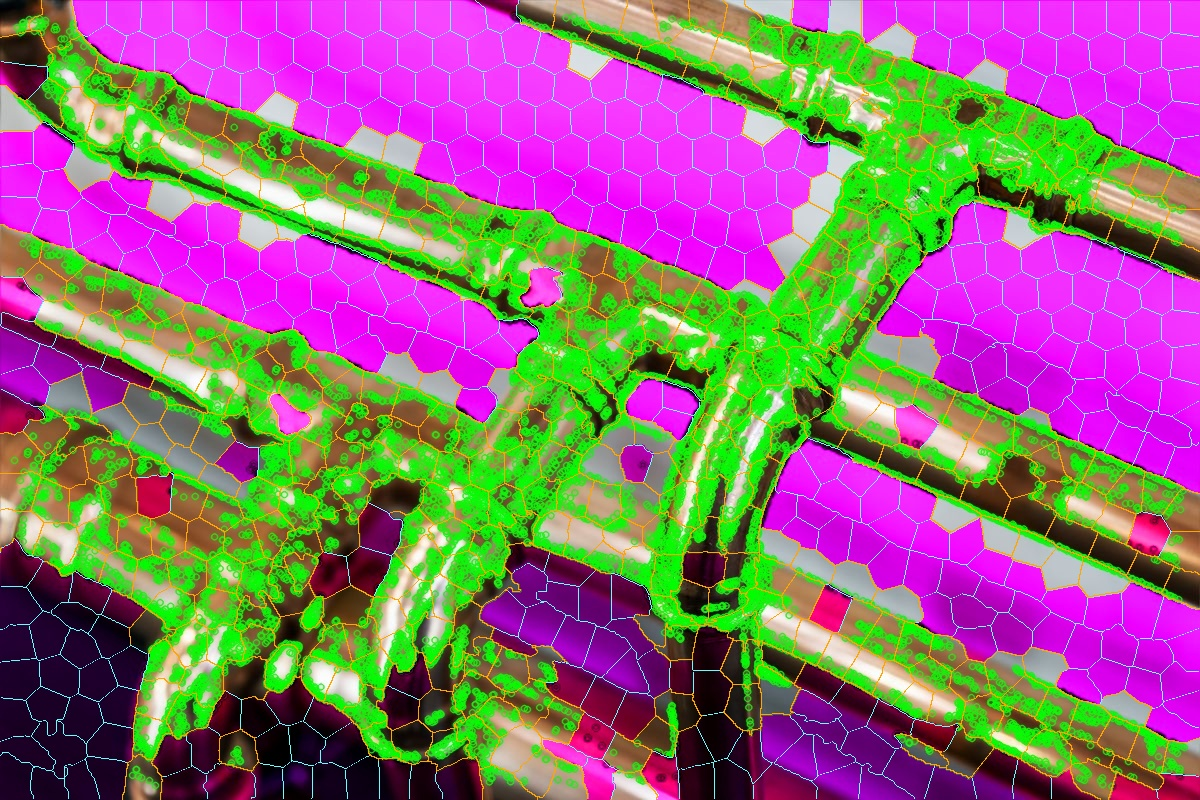
\includegraphics[angle=0.5,origin=c,width=0.4\textwidth]{pm/1.jpg}}}


\put(241,814){
	\transparent{1}{
		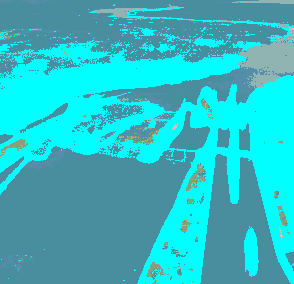
\includegraphics[angle=0,origin=c,width=0.31\textwidth,
trim=0 14mm 0 10mm, clip]{pm/7.png}}}


\put(452,828){
	\transparent{1}{
		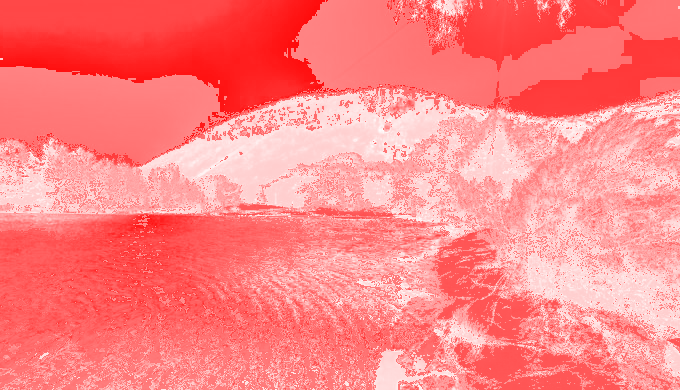
\includegraphics[angle=-1,origin=c,width=0.3\textwidth]{pm/2.png}}}



\put(442,797){
	\transparent{1}{
		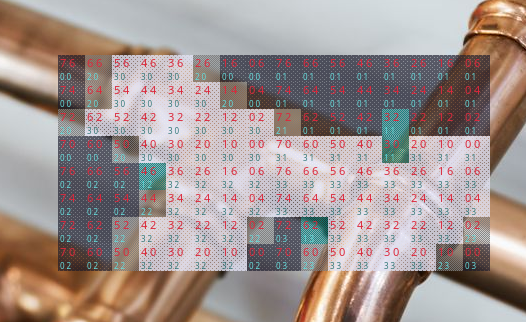
\includegraphics[angle=0,origin=c,width=0.18\textwidth]{pm/8.png}}}



% + 46
\put(12,588){
	\transparent{1}{
		
\includegraphics[angle=-0.5,origin=c,width=0.34\textwidth]{pm/3.jpg}}}

\put(52, 582){
	\transparent{1}{
		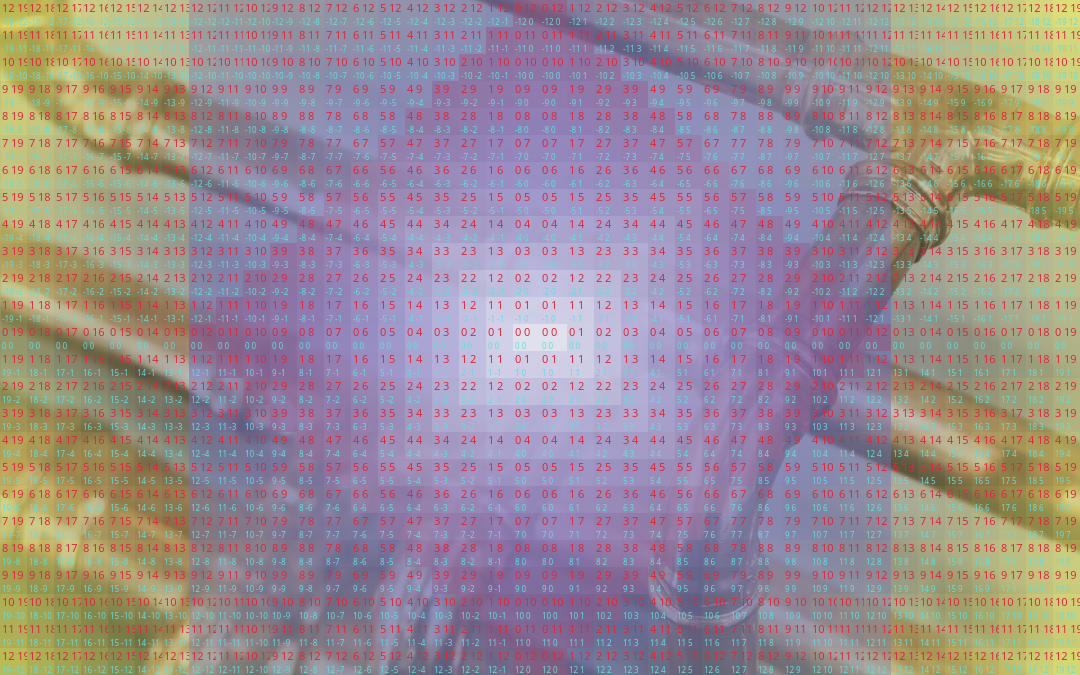
\includegraphics[angle=-0.5,origin=c,width=0.2\textwidth]{pm/6.png}}}

\put(402,578){
	\transparent{1}{
		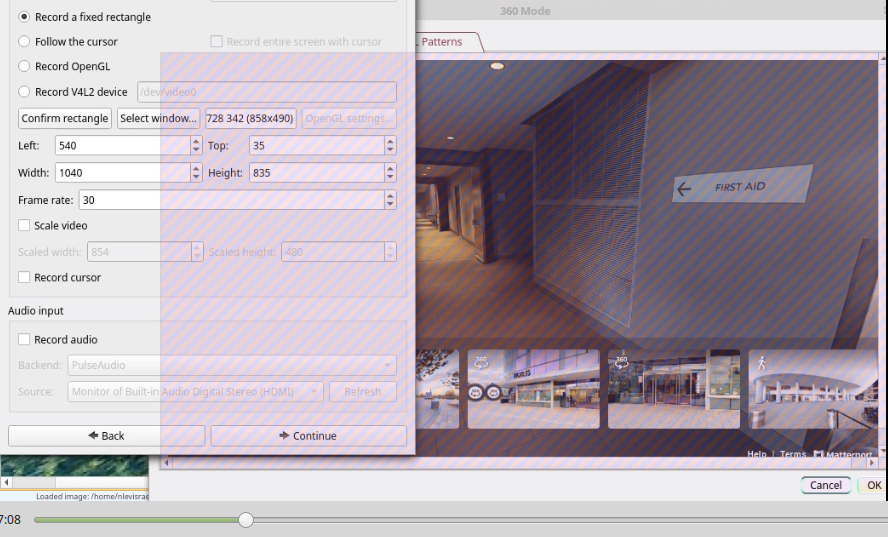
\includegraphics[angle=-1,origin=c,width=0.42\textwidth]{pm/5.png}}}



%


%\put(412,680){
%	\transparent{1}{
%		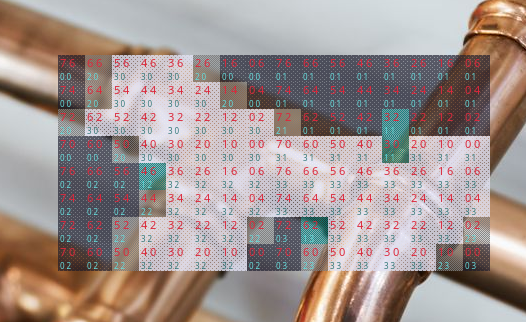
\includegraphics[angle=2.5,origin=c,width=0.2\textwidth]{pm/8.png}}}

%\put(402,407){
%	\transparent{1}{
%		
\includegraphics[angle=-1,origin=c,width=0.45\textwidth]{pm/3.jpg}}}

\fi
}	






\AddToShipoutPictureBG{%

\colorlet{redbl}{red!40!magenta}
\colorlet{yelbl}{yellow!60!magenta}

\colorlet{redblg}{redbl!30!black}

%\ifnum\value{page}=5{
%\AtTextLowerLeft{\raisebox{-5pt}{\hspace{5pt}\fontfamily{qtm}\fontsize{10}{11}\fontseries{b}\selectfont{}{\colorbox{yelbl!7}{\textcolor{redblg!70}{PLEASE SEE OUR SOFTWARE DEMO VIDEOS: \href{http://www.lingtechsys.com/videos/qmt-composite.mkv}{GIS},
%\href{http://www.lingtechsys.com/videos/dhax-composite.mkv}{360\textdegree{} photography}, and \href{http://www.lingtechsys.com/videos/xcsd-composite.mkv}{image processing}.}}}}}
%}\fi


}




\begin{document}

%\thispagestyle{empty}
\thispagestyle{firstpage}

\vspace*{83pt}

%\vspace*{1em}

\begin{center}

{\cyanhr}

\vspace*{8pt}

{\color{red!70!black}\fontfamily{phv}\fontseries{b}\selectfont

%\vspace*{13pt}

%{\Large{Solving the Machine Readable Problem}}

%\vspace*{10pt}

%{\Large{by}}

{\large{\llTorqAthreeR{}: Cloud Hosting Architecture and Web/Desktop Hybrid Software Engineering,}}

\vspace*{7pt}

{\large{as applied to Multimedia Government, Civil and Environmental Informatics}}

%\vspace*{7pt}

%{\large{Architecture, Construction, and Property Data}}

}

{\cyanhr}

\vspace*{38pt}

\hspace{-32pt}Amy Neustein, Ph.D.\\
\hspace{-32pt}CEO and Founder\\
\hspace{-32pt}Linguistic Technology Systems\\
\hspace{-32pt}Fort Lee, NJ\\
\hspace{-32pt}917-817-2184\\
\hspace{-32pt}\href{mailto://amyneustein@verizon.net}{amyneustein@verizon.net}

\end{center}

\vspace*{26pt}

%{\large{}}

%vspace*{6pt}


%}


\vspace*{32pt}

{\setstretch{1.1}


%\section{Overview}
%\vspace{}
\noindent\subtitle{{A New Cloud/Native Hybrid Software Engineering 
Framework for Embedded Web Applications,\\\vspace{3pt}  
Government Information Services,
Urban/Community Development, and Environmental Technology }}
%\sectvspace{}

\vspace*{5pt}

\vspace*{10pt}
{\semihr{0.093\textwidth}}
\vspace*{3pt}
%\sectnum{1.}
\hspace{2pt}\secttitle{{Introduction}}
\vspace*{5pt}
{\semihr{0.093\textwidth}}

\vspace*{4pt}

\p{Recently-developed technologies such as Cloud-Native hosting services, 
Embedded Web Sites, and Web/Desktop hybrid software applications present currently-untapped potential 
for next-generation civil and governmental information services --- particularly 
in the context of sustainability, Civil Engineering Informatics (\CEI{}), community development, 
and digital government.}

\p{Linguistic Technology Systems (LTS), a startup in Fort Lee, has engineered 
software components supporting next-generation information services with an emphasis on 
Translational Informatics --- a term used to characterize how science and 
research can be \q{translated} to benefits for individuals and communities, often abbreviated 
as \TRI{} (for \q{Translational Research Informatics}).  
We would like host governmental and/or civil data sets 
or multimedia resource archives which leverage 
and demonstrate this new technology.  LTS can set up the cloud-hosting infrastructure required 
for running services with the unique features described below.  For reasons explained below, 
most cloud hosts do not support the kind of Cloud-Native technology described here; 
as a result, a publicly-accessible cloud environment explicitly designed for such 
technology (with precompiled libraries and similar programming utilities) 
could be a beneficial public service, enabling developers to run software on the 
cloud that would be very difficult to deploy otherwise.}

\p{\lTRI{} and \q{Translational Science} was originally formulated in the context of bioinformatics 
and medicine, but more recently has been applied to other fields, including 
those related to climate change, environmental health, and public policy.  
We believe that \TRI{} protocols initially developed for tracking the progress 
of biomedical and pharmacological science \q{from bench to bedside} --- i.e., from 
the laboratory to beneficial clinical interventions --- can be adapted toward 
the documentation and analysis of scientific initiatives which, often through 
government actions, are operationalized toward community development and helping 
the environment.  Proper technology can support greater transparency and 
accountability for both government and science.  To this end, we have 
worked on a \TRI{} data-sharing and software engineering framework that 
we call \TorqAthreeR{} (Translational Research Query Protocol -- Application as a Resource)
with potential applications to civil/governmental data management.}

\p{In particular, we would like to develop a web service that could supplement and integrate governmental and environmental data for Bergen County and/or New Jersey as a whole, with an emphasis on environmental health, sustainable design, and civil engineering.  We propose to engineer this service with a focus on supporting web-site embedding into standalone, desktop-style computer applications, which is a relatively new way of accessing web resources.  Embedded web sites are used in specially designed standalone applications rather than visited exclusively via web browsers (although conventional browser-based access is still possible).  Web-site embedding allows web services to be enhanced with desktop-style technology that would not ordinarily be available browser-based web applications, such as showing multiple, interconnected multimedia windows simultaneously, or presenting isolated windows with structured data that complements content seen in a primary window --- for example, presenting details about a building or construction project in a dialog box appearing alongside representations of that building/site in a video, street view tour, or street map.}

\p{Code implementing \TorqAthreeR{} web sites/applications or services 
can be packaged and shared in a portable manner, so that the site may be run on multiple 
computers.  Simultaneously, \TorqAthreeR{} services are optimized to be accessed from self-contained, 
desktop-style software, using dedicated windows which render web pages essentially 
as miniature browsers, via technologies such as \smbf{QWebEngine} --- which functions as 
an instance of the Chrome browser local to a single (self-contained) application.  
When embedded in this manner, web sites/services can benefit from more sophisticated 
graphics, visualization and multimedia capabilities, exposed through the host 
application, than are possible through conventional (non-self-contained) browsers 
insofar as these expose a narrower range of functionality to intra-web application code.}

\newpage{}
\p{In general, sites which employ both 
browser-based and native functionality are known as 
\q{hybrid} applications.  Hybrids straddle the line between web and desktop paradigms.  
Engineering hybrid applications requires a software-development platform  
which is distinct from both the mainstream native frameworks (such as \Qt{} or 
\MFC{} --- Microsoft Foundation Classes) as well as the popular 
web toolsets (\smbf{Node}, \smbf{Rails}, 
\smbf{Django}, and so forth).}

%\newpage{}

\p{At the same time, once a shared instance of portable/multi-peer web applications 
becomes hosted in a public location (on the cloud, for instance), users can access \TorqAthreeR{} services 
without a local version of the relevant application on hand.  This includes both 
members of the general public who prefer not to download their own 
copy of the underlying software, as well as users who do have the software 
locally installed but will sometimes access the shared content from locations 
where their local program is unavailable.  The \TorqAthreeR{} model supports private 
data spaces where users can access their own specific content via a cloud share-point 
as if they were working from their own personal copy of the web service.}

\p{Likewise, common share-points can host data sets and resources that 
are too large for individual computers, such as \GIS{} tile servers (storing 
gigabyte-scale collections of digital-cartographic images, to create 
street maps and other \GIS{} rendering elements) and sizable arrays 
of video/multimedia files.  Similarly, functionality that is impractical to 
implement in a cross-platform manner may be encapsulated in a virtual application 
image (via technologies such as \smbf{docker}) functioning as a local web 
server, so that native front-ends are driven by back ends with their own 
virtual operating system.  Apart from use-cases where such virtualization is 
unavoidable, however, \TorqAthreeR{} could run as wholly native applications 
with the entire code base on a local computer, while simultaneously deploying a 
copy of the relevant server-side components on the cloud.}

\p{Overall, \TorqAthreeR{} combines several comparatively new technologies, 
such as \smbf{QWebChannel} or equivalent bridges 
to marshal data between web and native components; viewers (and parsers for 
metadata associated with) multimedia assets,
e.g., 360\textdegree{} photography or tile servers with detailed \GIS{} layers that 
can customize map-segment images to individual projects/applications; and \q{cloud-native} 
containerization for self-contained, native-compiled software instances.  
Perhaps because of these constructs' relative novelty (5-10 years, 
as compared to the 20-25 year span by now of \q{Web 2.0}) the infrastructure 
for supporting shared applications according to the criteria described 
here is not commonly available, by contrast (for instance) to 
ordinary cloud-native architecture supporting browser-based rather 
than embedded web sites.}

\p{For this reason, we encourage government initiatives which leverage 
hybrid-application and web-site embedding for next-generation civic/administrative 
information services --- with the added side-benefit of concretizing an 
infrastructure that could also be used by the public at large.  For example, 
cloud-hosting services with explicit support for hybrid/embedded web 
applications can be a publish-point for government web sites but, in so doing, space 
might be reserved for other kinds of applications maintained by 
private individuals or institutions, as an alternative to corporate 
cloud providers (e.g., Amazon Web Services, or \AWS{}).  Similarly, 
resources such as \GIS{} tile servers or government databases could 
be made available to the general public for a diverse range of use-cases 
(digital maps, for instance, benefit from customizable tile-server 
providers as an alternative to commercial programs, such as 
Google Street Maps, whose \GIS{} features are limited and 
occluded by practices that support their commercial business model; 
e.g., showcasing enterprises like stores or restaurants on map displays, 
whether or not these are relevant to the software where the maps are 
viewed).}

\vspace*{10pt}
{\semihr{0.27\textwidth}}
\vspace*{5pt}
%\sectnum{1.}
\hspace{2pt}\secttitle{{Web-Site Embedding and Multimedia}}
\vspace*{4pt}
{\semihr{0.27\textwidth}}

\vspace*{3pt}


\p{Web-site embedding is particularly useful in the context of multimedia databases where different media formats can be interconnected; e.g., geotagging video frames; linking \GIS{} map locations to videos or Virtual Tours of sites and buildings; or cross-referencing specific page-coordinate locations in \PDF{} files with map locations or with multimedia files.  Interactive cross-referencing provides enhanced, visually informative user experience, such as seeing urban/environmental redevelopment projects via \GIS{} maps, videos, Virtual Tours, and image-series in combination; however, this sort of user experience can only be achieved in a limited fashion in the browser.  Most web sites, however --- and, in fact, almost all web-development platforms --- are designed exclusively for browser-based access, and do not make any special provisions for use as embedded resources.  
To address these lacunae, we have engineered protocols to standardize how web sites may interoperate with host applications, allowing both sides to maximize web-site embedding's benefits.  Consequently, we would like to propose the curation of a government, civil engineering, sustainability, and environmental data web service that would implement these protocols when used as embedded resources, while also being accessible as ordinary browser-based applications.}

\p{In addition to superior user experience, web-site embedding allows host applications to unify several isolated web sites which are logically (but not logistically) interrelated.  This is particularly appropriate for governmental or environmental web sites, that tend to be artificially separated by jurisdictional boundaries.  For example, a researcher or governmental official interested in the environmental impact of municipal decisions --- such as sponsoring public/private initiatives or zoning and land-use classifications --- will find relevant data scattered across multiple websites partitioned by geographic boundaries.  New York City, other counties in the State of New York, and counties in Northern New Jersey each have distinct websites and their own offices for 
requesting information.  Maps such as NYCPlanning's \ZoLa{} system, which provides zoning and property info for the five boroughs, are blank across the river in New Jersey; while analogous resources such as New Jersey's Department of Environmental Protection (\NJDEP{}) interactive maps contain no information back in New York.}

\p{And yet, most environmental risk factors are shared between the states of New York and New Jersey --- hurricanes, flooding via the Hudson River or Atlantic Ocean, poor air quality, and so on --- and likewise housing and quality-of-life trends.  Unfortunately, however, because state agencies on opposite sides of the Hudson River operate separately from one another (and answer to disparate governments; Albany there, Trenton here) there is little incentive for New Jersey and New York State digital resources/platforms to be synchronized or interoperate.}

\p{Moreover, in the same way that useful data is often siloed in separate state and/or county web sites, important links between different kinds of multimedia content can be similarly neglected.  For example, maps, videos, image series, and virtual tours can all be used to showcase environmental restoration and/or urban-development projects, but most software applications have no way to connect different files which are interrelated --- for instance, connecting videos of a new construction project to interactive virtual tours of the same buildings.  The LTS software for \TorqAthreeR{} and \q{Translational Sustainability Informatics} (see below) addresses this problem by establishing a protocol for multimedia cross-referencing and providing software which can display diverse media types and follow cross-references so that users can browse between multiple interrelated file types.}

\p{Here are several examples of logical interrelationships that are meaningful when integrating diverse forms of multimedia in \AEC{} and \CEI{} contexts:}

\begin{description}[leftmargin=3pt, itemsep=-1pt]

\item[Building Inspections]  Companies which do residential and/or commercial building inspections 
--- including several in New Jersey --- have started to offer 360-capture photography as part of the 
inspection process.  360\textdegree{} photography produces virtual tours that can expedite 
initial or follow-up inspections, and document the history of a property's inspections, permits, and 
licencing.  Embedding virtual tours in desktop-style applications allows individual locations inside 
the buildings to be synced with government records, so users viewing the tour can seamlessly transition 
to accessing an inspections database (so as to research, for example, a commercial property's 
compliance with facilities codes, or the status of renovations). 

\item[Geotagging Videos]  Individual video-frames --- and in general the portions of a video 
running between two time-stamps --- can be annotated to declare that the 
video (at a given moment, or for a specified period of time) depicts or documents a real estate property or 
geospatial location with specific \GIS{} coordinates.  People watching 
these videos can then benefit from viewing them alongside interactive \GIS{} maps.  
Consider videos documenting environmental cleanup 
projects and rehabilitation of degraded land areas: while seeing the 
progress of a construction site, restoration of waterways, development of parts and 
other greenspace, etc., users can benefit from observing their positions on a 
map and noting relationships to surrounding streets, waterways, topography, and so forth. 
Special technology, however, is necessary to extract video-frame annotations and 
pass embedded \GIS{} data and coordinates to geospatial displays --- and, in general, 
to develop computer software where \GIS{} maps and video players co-exist in one application.    

\item[Converting street-view or virtual tours to video]  Virtual tours allow users 
to select their own (digital) path through a building or outdoor site, but for some purposes 
it can be helpful to run a tour with a specific path selected for demonstration and 
documentation purposes, and then capture the results as a video that may be 
replayed with no changes to the walk-through 
(such video-capture also requires special-purpose software).  Street-view 
tours of an urban neighborhood can likewise be converted to videos, which 
can be useful for similar reasons. 

\item[Emergency Management and Hazard Mitigation]  Cross-referencing digital maps with videos, 
photo galleries, and/or virtual tours can document how jurisdictions identify and 
mitigate environmental and/or public risk factors.  For example, maps and videos 
(including those derived from street views) might jointly show flood or fire evacuation 
routes; identify industrial sites where there exists a contamination risk, or similar 
public health concerns; document patterns of erosion, drought, floods, soil change, and 
similar indicators of climate change having an effect on local ecosystems; and track 
potential ecological antagonists such as invasive or harmful species (e.g., 
toxic algae).

\item[Government Services]  Syncing maps with government data sets can make it easier to 
provide information about public services to residents of (or visitors to) local 
communities.  For example, a single portal which loads public transit data alongside 
maps and street views can help phone operators direct customers to their correct 
bus stop, in locations where there are several nearby stops serving different 
routes; or where customers need stops with or nearby specific facilities, 
such as a seating area, a location to buy tickets, or a convenient waiting place 
(e.g., a restaurant or coffee bar).

\item[Zoning and Land Use]  Adapting digital maps as an entry-point for 
obtaining information about zoning, land use, residential/commercial 
property data, local ordinances, and so forth, can expedite public use of government databases.  
For example, Zoning and Land Use maps could be linked with photos, videos, 360\textdegree{} photo assets, 
or \PDF{} files which visually and/or interactively explain the restrictions/requirements 
enforced for locations within different land-use areas.  
Relevant documentation could then be loaded directly from \GIS{} coordinates based on the 
zone classification of a selected \GIS{} location.  In the case of \ZoLa{}, for example, 
New York City residents can open a small box summarizing the definition of the 
applicable land-use designation for any map location, but further details about 
the relevant zoning regulations are only available from a separate part of the 
web site.  A more multimedia-oriented front end (using an embedded web site) can 
load a \PDF{} document or a video explaining the local zoning parameters 
directly from the digital map, superimposing it over the map window near the specified 
\GIS{} coordinates.          

\item[Track Social and Development Trends]  Embedding interactive maps with 
data sets that show timelines or historical data about trends such as 
population changes, urban renewal projects, 
patterns of construction and community development, or impacts of environmental policy, 
can help to document and assess the influence of municipal, county, or state 
laws/regulations and initiatives on environmental well-being and quality of 
life.  In particular, insofar as jurisdictions might cite specific 
(quantifiable) metrics for government policy --- acknowledging parameters 
such as optimal population density, housing availability, low carbon-footprint 
construction, reductions in air/water pollution, improved traffic flow, etc. 
--- multimedia data sets and presentations can document the effectiveness 
of programs or regulations at meeting their declared goals.  It is one thing, say, 
to state in words a jurisdictions' commitment to ecological cleanup/restoration or 
the construction of new residential properties; but a more convincing presentation 
will actually document the sites and locales affected by such policies 
with pictures, videos, or virtual tours.  Indeed, quantifying the effectiveness 
of policies adopted for ecological and/or community-oriented reasons serves an important 
role of clarifying how well scientific models of environmental health and sustainability 
are \textit{translated} to concrete societal action, continuing 
the analogy with \q{translational medicine.} 
     
\end{description}


\p{We believe that governments, researchers, and the general public deserve an integrated portal which aggregates data about climate change, environmental factors in public health, and sustainable engineering and design solutions with demonstrable social and ecological benefits.  Data integration is especially important because health, environment, energy, and civil problems and solutions are tightly interconnected.  For example, problems exacerbated by global warming  --- such as toxic algae blooms --- cause ecological damage (polluted waterways) that in turn yield public health risks (cyanobacteria poisoning) and economic harm (via agricultural damage).  Likewise, local government policy (such as zoning and land use classification) shape population density and traffic flows, which in turn affects air quality, energy consumption, and carbon emissions.  At the same time, sustainability initiatives --- such as Superfund designations --- have positive impacts that branch in multiple directions, including better environmental health (both through removing pollutants and transitioning former industrial areas to natural, potentially carbon-sequestering habitats) and social/economic benefits as superfund sites are redeveloped (parks and natural areas for quality of life, and/or residential or commercial areas for economic benefit).  These are a few examples of converging energy/environment/ecology/engineering/economic factors.}

\p{Consider the following scenario: someone intends to study land-use patterns in the context of global warming and natural hazards; specifically, how to formalize the assessment of hazard risk relative to different zoning classifications (industrial, commercial, residential, with different population-density averages).  There are several data sources which would be logical places to acquire relevant information, including the \ZoLa{}, \NJDEP{}, and the World Food Programme \PRISM{} \q{climate risk monitoring} project, which receives Earth Observation data and cross-references it with \q{information on socioeconomic vulnerability ... to inform disaster risk reduction and social assistance programmes.}  In this hypothetical example --- merging land-use and hazard-risk data for both states via the \PRISM{} system --- the three specific components involved (\PRISM{}, \ZoLa{}, and \NJDEP{}), although each operate via an interactive \GIS{} interface, are technologically incompatible; there is no way to merge data from one map onto either of its peers.  The \ZoLa{} display shows no land-use data for New Jersey, and vice versa for \NJDEP{} \visavis{} New York; and neither map can show \PRISM{} data layers}


\p{In general, information curated at local, state, and government levels which pertains to collective 
environment/engineering/economic factors tends to be piecemeal and fragmented, failing to recognize the factors' interconnections.  Data which is overlapping and jointly relevant tends to be split among disparate web sites and databases with no cross-referencing, data-discover mechanisms, or acknowledgement of important inter-relationships.  To illustrate this problem in concrete terms, here is an example of several governmental and environmental resources specific to Northern New Jersey:

\begin{itemize}

\setlength\itemsep{1pt}

\item{} New Jersey Department of Environmental Protection:  \NJDEP{} provides a collection of interactive maps which support visualizing and querying various data sets related to environmental protection, wildlife, agriculture, pollution, and related ecological details.

\item{} NJ-MAP, developed by Rowan University, provides interactive maps covering a range of domains across both natural and urban/governmental data sources, such as New Jersey Conservation Blueprint (resources specific to protecting natural land areas) and a Parcel Explorer that aggregates geographic and land-use data for individual property lots.

\item{} NJADAPT, part of the Climate Change Resources Center at Rutgers University, provides maps and data-visualization for studying the effects of climate change on New Jersey communities, addressing both natural and man-made ecosystems.

\item{} New Jersey Division of Water Monitoring \& Standards (\DWMS{}), in conjunction with Rutgers University, provides interactive maps with a \q{Continuous Data Monitoring Program} yielding a frequently-updated publicly-accessible portal specific to hydro-ecology.
  
\item{} County-Level Offices of Emergency Management (\OEM{}), as well as the state-level \OEM{}, are responsible for curating and sharing information about natural and man-made emergencies.  This includes a \FEMA{}-mandated Hazard Mitigation Plan, typically developed individually within each county with data aggregated from each jurisdiction, that requires local governments to document the steps they are enacting to help prevent loss of life or property damage in the event of natural disasters and other hazards.

\item{} The National Institutes of Environmental Health Sciences (\NIEHS{}) provides a suite of tools for publishing information connecting environmental and public health, ensuring that data from disparate sources becomes interoperable and collectively analyzable.  This includes a \q{translational research} framework organized in concentric \q{rings} progressing outward from biomedical/biochemical investigations to public health and environmental policy.  Likewise, \NIEHS{} established an \q{Environmental Health Language Collaborative} to define a common format and semantics for asserting environmental and public health observations and data sets, including those relevant to describing environmental hazards and mitigative steps such as those addressed by Hazard Mitigation Plans. 

\item{} \ZoLa{}, New York City's Zoning and Land Use information service (mentioned earlier) was implemented on top of an innovative code library for \GIS{} web services, called Ember Mapbox Composer, that itself was developed and published by NYCPlanning.  Although \ZoLa{} is specific to New York City, Ember Mapbox Composer is independent of any particular database or jurisdiction, and could be reused by other cities and states.

\item{} \PRiSM{} (Precision Manufactured Housing), a project developed by the city of London (UK), is a tool to spearhead sustainable \AEC{} practices in the London metro area (note that this \PRiSM{} is unrelated to the \PRISM{} portal, referenced above, curated by the World Food Programme).  \PRiSM{} tools include \GIS{} and \CAD{} displays as well as charts/plots and other data-visualization resources relating to civic \AEC{} data in the London region.  Although specific to London (the city did not provide a generic back-end analogous to Ember Mapbox Composer as the technology behind \ZoLa{}) it is probable that other cities could benefit from applications modeled around \PRiSM{} (perhaps multiple cities could collaborate to create a version of \PRiSM{} not tied to London 
or any other particular geographic location).


\item{} The other \PRISM{} --- the one implemented by the World Food Programme (\WFP{}) -- is also a useful resource for risk/hazard mitigation due to environmental factors.  The backstory behind this \PRISM{}, insofar as it was spearheaded by an organization whose stated purpose involves combating global hunger instead of climate change, was the \WFP{}'s recognition that climate change exacerbates the socioeconomic stress factors which contribute to nutritional insecurity.  The organization therefore built \PRISM{} with the explicit purpose of pairing socioeconomic data with environmental observations, using domain-specific techniques to extract socioeconomically salient data sets and trendlines from Earth Science observations (correlating droughts with food shortages, for example, or quantifying how climate change affects internally displaced persons and emigration).  \PRISM{}, in turn, receives environmental data from the Committee on Earth Observation Satellites (\CEOS{}) via Open Data Cube (\ODC{}), a platform with multiple domain-specific instances, including the \WFP{}'s \q{Humanitarian Data Cube.}  Other initiatives, such as the Climate Hazards Center (\CHC{}) at the University of California -- Santa Barbara, employ a similar analytic framework, and the Humanitarian Data Exchange project, via Humanitarian Exchange Language (\HXL{}), offers tools for merging thematically connected data sets such as those from \WFP{} and \CHC{} to augment each other's scope and detail. 

 
\item{} The Institute for Sustainable Infrastructure (\ISI{}) \q{envision} framework models 64 \q{sustainability and resilience indicators,} also called \q{credits,} which document sustainable practices adopted per-project by entities in the Architecture, Engineering, and Construction (\AEC{}) sectors.  The World Resources Institute (\WRI{}) \q{\ZCB{} Pathways} framework is a similar method for tracking progress toward \ZCB{} (Zero-Carbon Building) emissions goals.  By applying the \ISI{} and \WRI{} models to new or existing buildings in their communities, local and state governments can document how they are addressing climate-change related risks by reducing buildings' energy use and carbon footprint.  The significant detail about \ISI{} and \WRI{} models is that, in additional to generic \q{best practice} recommendations, they have also formulated specific metrics, assessment tools, and iconography which quickly documents how extensively and in what manner buildings adopt sustainable practices, making it possible to aggregate data from multiple properties into a more holistic model of trends in the context of specific locales and communities.  For instance, \ISI{} or \WRI{} icons can be employed in \GIS{} maps; a higher concentration of icons in given localities indicates that \AEC{} firms in that area (perhaps with influence from local governments, via leveraging tactics such as land-use abatements or public/private partnerships) have embraced sustainable practices within multiple sites and projects.   

\end{itemize}
}

\p{The concerns addressed by each of these projects or organizations are overlapping and in many ways mutually reinforcing.  For example:

\begin{enumerate}[leftmargin=3pt]

\setlength\itemsep{1pt}

\item{} Identifying environmental risk factors overlaps with emergency management, insofar as general threats due to ecological damage can transition to emergencies demanding immediate responses in the wake of natural events or human accidents.  For example, polluted waterways (due to toxic algae, as mentioned earlier, or due to industrial chemicals) that present a baseline threaten to human or animal health in their vicinity can become more hazardous due to storms or floods that cause the waters in affected areas to spill over into rivers, aquifers, and other usually safe waterways.  Similarly, industrial sites containing dangerous materials present a public health hazard in the event of forest fires.  Data for tracking sites with long-term environmental-health consequences will intrinsically, therefore, overlap with formulating protocols for occasional emergency management.  Conversely, improving sites presenting long-lasting pollution threats is an effective form of hazard mitigation and risk reduction/management.

\item{} Sustainable architecture and engineering categories developed by the \WRI{} and \ISI{} are associated with specific buildings, land-areas, and construction projects.  Both \WRI{} and \ISI{} offer a series of terms and icons that indicate sustainable practices adopted at specific locations; because these indications are tied to geographical locations, they can be incorporated into \GIS{} maps addressing environmental and climate-change factors.  Mapping the adoption of sustainable practices can help to visualize trends in where such practices are being applied more thoroughly (which communities are especially forward-looking in this regard) and can document relationships betweens regions that embrace (or lag behind \visavis{}) sustainable \AEC{} and areas projected to be most affected by climate change (flooding, forest fires, rising ocean levels, etc.)
 

\item{} Zoning and land-use classifications, which are typically the responsibility and under control of local jurisdictions, have a significant effect on the climate footprint of urban and suburban communities --- affecting traffic patterns, concentrations of population density, and environmental impact of industrial development, plus the consequences of clearing natural land for construction in the first place.  Municipalities may choose to alter zoning policies either holistically or on a case-by-case basis, under the influence of environmental impact studies; in some cases governments might offer abatements for individual developers who propose projects with direct social/environmental benefits --- such as well-situated residential units --- or eco-friendly enhancements, such as commercial developments paired with greenspace-preserving parks or publish-use areas.  Digital records can document zoning and land-use decisions and proposals, along with relevant data and analyses, adding greater transparency to this process and also encouraging neighboring districts to work in consort toward sustainable Civil Engineering practices. 

\item{} Multi-Media technology is important for presenting sustainable \AEC{} solutions.  Sustainability in Architecture and Construction addresses several facets of building design, including physical materials, cost-effective construction techniques, and energy efficiency post-occupancy.  Organizations such as \ISI{}, \WRI{}, and the International Institute for Sustainable Development (\IISD{}) --- alongside localized projects such as London's \PRiSM{} software --- provide \AEC{} recommendations across these design areas.  However, such documentation is often cursory and hard to visualize; for example, it is difficult to find videos or virtual tours showing sustainable-engineered buildings from a practical perspective.  In the case of Precision Manufactured Housing 
(\PMH{}), say --- which is a promising new technology for cost-effect \AEC{} implementation --- it is difficult to visualize what \PMH{} buildings look like, what the experience is like to live or work in them, and so forth.  Similar comments could be made about \q{smart building} techniques using designs and materials (such as natural cooling) to reduce carbon footprint.  Multi-Media presentations can help by syncing image series, videos, and virtual tours with \TwoD{} floor plans or \ThreeD{} \CAD{} presentations: 
having the opportunity to see sustainable \AEC{} techniques formulated within \CAD{} software and then transition to seeing the real-life results, via video tours showcasing buildings, or virtual building walk-throughs, with sustainable design features and materials highlighted via annotations and/or supplemental documentation.  In the case of modular \PMH{} design, for instance, what are the individual building parts; how do they look pre-assembly versus on-site; how do modules piece together into an organically holistic design; and how can \q{smart} features be showcased insofar they are installed and utilized in a completed building?     

\item{} Eco-friendly \AEC{} practices need to be evaluated in conjunction with sustainable land use patterns.  \q{Green} \AEC{} can promote sustainably-sourced and/or energy-efficient buildings from a site-specific point of view, but \AEC{} environmental impact is also more holistic.  For example, construction projects which disrupt natural habitats and/or are poorly connected to local neighborhoods and transit routes (causing, e.g., longer car commutes to nearby cities) can have a net negative impact even if the buildings themselves are designed in an eco-friendly manner.  The domain of \q{sustainable} architecture includes using building materials and designs which minimize environmental footprints both when sourcing construction and post-occupancy, but this domain also involves construction protocols that offset the exceptionally high \AEC{} costs typical of US urban areas.  In the best-case scenarios, new buildings will simultaneously optimize sustainable design, construction cost relative to the number of residential units created, and integration with local communities and transit options (e.g., siting eco-friendly buildings on underused lots close to urban centers is more eco-friendly than comparable exurban projects).  Correctly analyzing these multiple optimizations factors requires cross-domain data integration.

\item{} Government incentives, such as Superfund designations and public/private collaborations, are generally assessed for both their environmental and economic benefits.  Therefore, metrics for defining project goals, and subsequently performance evaluations, call for quantification of both environmental and economic impacts, as well as integrated information sources providing the requisite data in each domain.  From the public's perspective, for example, \GIS{} services mapping out Superfund and/or public-private codevelopment sites can link each site to documentation of the commercial entities that stand to benefit from the projects (and that are accountable for ensuring that projects actually show their anticipated positive outcomes) as well as environmental-impact projections. 
\end{enumerate}
}

\vspace*{-1em}

\p{As these examples suggest, sources which provide information within one specific domain (such as \AEC{}, environmental data, zoning and land use, Civil Engineering, and so forth) are most valuable when they can be cross-referenced with interrelated data addressing parallel concerns, linked by \GIS{} coordinates, municipality, or initiatives (for instance, multiple Superfund sites across Bergen, Hudson, and Passaic counties; or Superfund locations in one borough linked to other climate-mitigation projects within the same jurisdiction).  Our proposed dashboard and database would operationalize such data-integration by unifying multiple data-sources both at the User Interface level and via a multi-source data query mechanism.}

%
\p{In general, this kind of data synthesis proceeds along two parallel tracks, source-integration and application-integration.  Application Integration means providing one single application which allows users access to multiple data sources.  For this proposal, we envision a single self-contained desktop-style application that would embed websites such as those listed earlier (and any other ones which are relevant) as well as free-standing map views, images, charts/data-visualization, videos, 360-photography tours, and other multimedia assets.  Users could switch between multiple data sources or view them side-by-side.  To support multi-source interoperability, the host application would define a common protocol for user interactions with each of the interconnected web sites and data back-ends.  Data-Source Integration, conversely, involves constructing or stacking \API{}s, \ABI{}s, and other integration layers to ensure that disparate data sources can be accessed via common data models, access protocols, and query systems.  Wherever possible, such integration would extend existing sources' capabilities (such as \API{}s) to honor Common Data Models and other type- or query-level protocols designed to merge multiple source-points into a common information space.  When directly modifying data-sources is not possible, adaptation layers can be introduced to translate common protocols into \API{}/query requests that the underlying data source can recognize.}


%\newpage{}

%\newpage{}
%\newgeometry{top=1in, bottom=.75in, left=.6in, right=.6in}
%\pagestyle{default}

%\vspace*{-38pt}

%\sectprevspace{}
%\sectnum{1.}\secttitle{{Translational Sustainability Informatics}}
%\sectvspace{}

%\vspace*{1em}

\vspace*{10pt}
{\semihr{0.32\textwidth}}
\vspace*{6pt}
%\sectnum{1.}
\hspace{2pt}\secttitle{{Translational Sustainability Informatics}}
\vspace*{4pt}
{\semihr{0.32\textwidth}}

\vspace*{5pt}


%\begin{minipage}{\textwidth}
\p{Taking inspiration from \q{bench-to-bedside} research in Translational Medicine --- referring to the \q{lab bench} and in general the steps requisite for translating biology and bioinformatics to concrete clinical practice --- Translational Sustainability encompasses tools and perspectives needed to leverage contemporary science toward sustainable and eco-friendly human communities.  In the context of computer software, Translational Sustainability emphasizes tools related to \AEC{} and \CEI{}, particularly towards the goals of designing \q{green} residential, commercial, and industrial buildings; environmental cleanup; and successfully integrating social and environmental concerns via urban planning (increasing housing density while decreasing car traffic, for example, or creating parks and nature-preserving spaces that benefit the environment as well as public health/quality of life).}
%\end{minipage}

%\newpage{}

\p{The term \q{Translational Sustainability} is sometimes used (e.g., by a University of Michigan research center) to describe investigations into translating scientific results in fields such as ecology, chemistry, and materials science into practical uses for eco-friendly and sustainable \AEC{}.  This is one of several recent scientific disciplines described as \q{translational} by analogy to clinical medicine.  Analogously, \q{Translational Informatics} addresses the overlap of computer science with translational research in disparate domains, with respect to data warehousing, integration, and analysis --- again inspired by biomedical practice (bioinformatics) but generalizing to science in general, alongside \CEI{}, geoinformatics, cheminformatics, etc.}


\p{Our interest in Translational Sustainability is focused on using multimedia software engineering to plan and analyze sustainability initiatives.  More generally, multimedia software improves the overall ecosystem of civic data managed by governments at different levels, from individual towns and cities upward.  We are committed to developing software which synthesizes and cross-references different kinds of multimedia content, in contrast to most current software applications, which will typically handle only one or two media types.  Integrated multimedia software allows users to access diverse multimedia content, and multiple embedded websites, at one time, which is more convenient from switching between applications and/or websites even if their content is inter-related.}

\p{We suggest the hybrid phrase \q{Translational Sustainability Informatics} 
(which could be abbreviated as \q{\TSI{}}) to express the intersection of 
\q{Translational Sustainability} and \q{Translational Informatics} --- 
focusing on data management and Software Engineering in the 
Translational Sustainability context.  
\lTSI{} can combine implementations in several areas, particularly these:

\begin{enumerate}[leftmargin=3pt, itemsep=-1pt]

\item{} Environmental Science:  Assessing how measurements of environmental health/degradation and climate change --- plus simulations of future climate conditions and the climatological effects of human activities and man-made materials --- can inform proper steps for mitigating our deleterious effects on the environment.  For example, ecological data can document trends before and after climate-mitigation interventions.

\item{} Health Science:  Documenting effects of toxins, pollution, and climate-related hazards (such as algae blooms) to human and ecosystem health via biomedical technologies.  The \NIEHS{}, for example, is a subdivision of the National Institute of Health; much of the former's research addresses modeling the effects of ambient toxins on cells and organ systems, and measuring or simulating such effects via bioimaging, in-vivo/in-vitro experiments, digital reconstructions, and so forth.  Epidemiological data can also track environmental effects on human populations as a public health concern.

\item{} Architecture, Engineering, Construction, and Sustainability:  Exploring how fields such as materials science, architectural physics, energy-efficiency, and industrial manufacturing can yield practical \AEC{} tools which optimize building's cost-effectiveness both in terms of progressing through planning, design, and construction phases and post-occupancy.  Examples questions include how to apply modular/prefab or \DfMA{} (Design for Manufacturing and Assembly) techniques to reduce construction costs, and how to achieve natural cooling, ventilation, shade, solar heating, and other organic connections with buildings' environment to mitigate the need for electricity to create comfortable living conditions.

\item{} Civil Engineering and Sociodemographics:  \lTSI{} can overlap with Civil Engineering Informatics (\CEI{}) and related information-management strategies, particularly in the context of governance and urban development.  Analyzing population trends and socioeconomic data, for example, can clarify the relationship between urban communities and their surrounding natural ecosystems.  Environmental conservation strategies will necessarily be different in medium-to-high density urban areas --- with small land-areas dedicated to greenspace that are integrated into residential and civic infrastructure --- compared to more distant rural and exurban zones.  Societal trendlines can also impact connections across the boundary between human and natural environments: for instance, a shift toward remote office work (and away from commuting) can have the positive benefits of less car traffic, but it also points to concerns about sustainable infrastructure closer to where workers live --- widening the area where eco-friendly and community-oriented civic development strategies are important outward from office-centered downtowns to cover large swaths of metro areas.  

\end{enumerate}
}

\vspace{-7pt}

\p{Like many \q{informatics} disciplines, \TSI{} can be focused on formalizing canonical representations for data sharing and reuse.  Bioinformatics, as an example, often concentrates on standardized encoding for genomic data (gene sequences, transcriptomes, mutation-evolution) and preserving/annotating diagnostic images; canonical genetic and picture-archive formats ensure that information can be shared across many different access points (multiple hospitals, research centers, diagnostic labs, etc.).  Similarly, geoinformatics is structured around the common reference point of geographic coordinates, through which any data with geospatial components can be cross-referenced --- most familiarly via latitude and longitude, but \GIS{} systems also often use other \GIS{} units, such as those based on tile-map renderings or Mercatur projections.  Geoinformation technology needs to properly annotate information source to indicate which coordinate systems are employed for any given data set (and also provide algorithms for inter-converting between systems, e.g. latitude/longitude to Mercatur formulae).  \lTSI{} can similarly focus on standardized data-representation techniques, coordinate systems, units of measurement, dimensional analysis, and related protocols to ensure interoperability between data sources representing the distinct scientific concentrations feeding in to Sustainability research (ecology, sociology, engineering).}

\p{As with other informatics branches, the proper role for \TSI{} involves best practices formulated for reusable software and application packages --- in short, code models and protocols alongside data models.  For one concrete example, consider sustainability documentation in the context of modular architectural design.  
Controlled vocabularies, such as those proposed by \ISI{} Envision and the \WRI{} Zero-Carbon framework, or similarly the \NIEHS{} Environmental Health Language Collaborative, define standards which software should adopt when serializing and describing data for sharing with other software components.  
However, similar semantic requirements come to the fore in the 
context of software application design in the first place.  
There are, for example, plugins to \CAD{} programs which are used to design modular-housing units; such plugins allow \PMH{} (precision-manufactured housing) or \DfMA{} data models to be recognized and visualized within \CAD{} front-ends, and incorporated into calculations alongside other \BIM{} (Building Information Management) and \IFC{} (Industry Foundation Classes) profiles.  This is not only a data-sharing issue, but also affects the \CAD{} User Experience directly; the design screens for \PMH{} units, say, would be enhanced to incorporate user-visible icons and options for loading \TSI{}-specific data-entry/summary forms or algorithms/computations (for example, calculating cost-per-unit for \PMH{} manufactured components, or visualizing how multiple modular component are interconnected in a completed building).}

\p{In short, we envision an application-oriented \TSI{} information model that defines protocols for managing \TSI{} data within user-visible applications (including \CAD{} programs, blueprint viewers, property-management software, and Civic Data engines such as \PRiSM{}) as well as inter-application data sharing operating more behind-the-scenes (i.e., typically not user-visible).  The \TSI{} protocols in this sense can address such concerns as systematic description of user-generated events when viewing \TSI{} data and/or \UI{} components; populating \UI{} components with \TSI{}-related data types; icons and terminology for identifying \TSI{}-specific data and operations in the context of software which is not specific to \TSI{} (e.g., \CAD{} and \AEC{} technology); and standards for representing \UI{} state when sharing data across applications.}


\vspace*{10pt}
{\semihr{0.26\textwidth}}
\vspace*{6pt}
%\sectnum{1.}
\hspace{2pt}\secttitle{{PDF/SVG Formats and Text Mining}}
\vspace*{4pt}
{\semihr{0.26\textwidth}}
\vspace*{4pt}


\p{Earlier comments about multimedia cross-referencing also apply to 
text documents and, by extension, digital text readers, such as 
\PDF{} viewers.  Renderers for \PDF{} files 
do not usually interoperate with multimedia software, 
so that for example a user could not in general click on a chemical 
formula referenced in a research paper and then have an option 
of viewing a corresponding molecular-\ThreeD{} model --- even if the 
research text and \PDB{} (Protein Data Bank) or 
\SDF{} (Structure-Data File) formats coexist in 
one overarching data set.  The \TorqAthreeR{} system 
incorporates a hybrid \PDF{}/\SVG{} format whose goal 
is to integrate \PDF{} viewers with multimedia 
components.  This format works somewhat by analogy to \GIS{} systems: consider 
a \PDF{} page as akin to a digital map at moderate-to-high zoom levels; 
then sentences are like city blocks or avenues, \PDF{} page 
coordinates are analogous to latitude/longitude, 
and sentence boundaries could be highlighted via 
geometric formations analogous to shape files.  
It is easy to direct readers toward a specific 
page in some other publication, but it is harder to 
create a reference to a specific \textit{paragraph}, or 
\textit{sentence}, or even the occurrence of one 
specific technical \textit{term} or Named Entity in a different 
(or even the same) document.  The example of 
geotagging is useful as a point of contrast: latitude and longitude 
coordinates (or other \GIS{} parameters, such as so-called 
\XYZ{} triples based on a global Mercatur projection) can be 
specified with arbitrary precision, so it is possible with one 
consistent tuple of numbers to unambiguously refer to 
a precise point on (or at some elevation above or below) the 
Earth's surface.  Any kind of media (text, images, videos, etc.) is 
able therefore to embed links toward \GIS{} maps merely by geotagging 
specific entities.  The \GIS{} case is unusual, however, 
in that the entire geoinformatics field is centered on 
one specific spatial domain (viz., Earth's surface); most 
data spaces do not have comparable universal coordinate-systems.  
For example, we can cite one specific page within a text 
document (which is, perhaps, roughly equivalent to city or 
county, in the cartographic realm), but we cannot (in general) 
designate individual points \textit{within} a single text page.}

\p{Via a \PDF{}/\SVG{} hybrid, however, metadata could 
cite locations internal to a document page within the 
scale of fractions of a typographic 
point, similar to latitude and longitude coordinates 
on a map.  When displayed, \PDF{}/\SVG{} files thereby 
become interactive: regions such as page-areas spanned 
by sentences, paragraphs, or smaller text segments 
(the character-range within a technical term, 
keyword, acronym, or other Named Entity, for example) may be 
assigned unique \SVG{} identifiers and take on 
distinct visual representations, as a cue to the 
user that these specific areas have special interactive 
possibilities.  For instance, sentences might be highlighted 
when the mouse hovers on their interior, indicating that 
the sentence as a whole responds to mouse events; 
e.g., a context menu whose options might include 
copying the sentence text (to the system clipboard, or perhaps a 
digital scratch/\q{notes} pad).  
This is more convenient than the current convention, where 
text segments are copied by 
laboriously positioning the cursor at the 
first letter in a sentence and then dragging the 
mouse to the end (usually just beyond a closing 
period or other punctuation mark).  That kind of 
extended user action can be replaced with a single 
click, given proper text-encoding and cross-referencing 
between encoded text-segments and \PDF{} page coordinates.}

\p{Text mining and open data sharing  
have both emerged as key facets of contemporary 
scientific research, for related reasons: 
text mining and data transparency are both 
techniques for expanding the scope of individual 
research projects, maximizing the potential 
for insights and discoveries made possible by 
pooling multiple projects' data and methodology.  
However, existing research-oriented technologies reveal 
limitations that have prevented text mining and 
data transparency from benefiting science to their 
full potential.  Key limitations include: 
flawed transcription of scientific text into machine-readable 
documents that are suitable for automated text mining 
tools; lack of sufficient structure within published 
data to fully implement protocols related to 
microcitations, \q{nanopublications,} and other 
strategies for designating and tracking the provenance 
of fine-grained data aggregates within larger-scale 
research environments; and the absence of rigorous 
protocols for integrating and cross-referencing data 
and text across different media and genres, including 
scientific literature and raw data sets along with 
multimedia resources (videos, \ThreeD{} models, 
\GIS{} maps, image-series, etc.).}

\p{The limitations of existing scientific-publishing technologies, 
in particular, became especially evident during the \smbf{Covid19} 
pandemic, when scientists sought to unify 
research across many distinct disciplines --- from 
epidemiology and virology to clinical data, and biomolecular 
analysis of the \smbf{SARS-COV-2} infection mechanism.  
A good example of the interdisciplinary response during that 
early-pandemic phase was the \CORDNineteen{} corpus (\q{\smbf{Covid19} Open Research Dataset}), 
curated by the Allen Institute for Artificial Intelligence (\AItwo{}).  
This project made thousands of papers about Coronavirus biology 
freely available, but also compiled structured versions of all 
articles into a machine-readable format --- encouraging programmers 
to develop text mining and/or \AI{}-based tools for 
analyzing the corpus in its entirety.  \CORDNineteen{} helped  
spotlight limitations of existing publishing technology: as we 
reviewed in a 2022 book about \smbf{Covid19} (as well as cancer and cardiac 
bioinformatics\footnote{\textit{See} \href{https://shop.elsevier.com/books/innovative-data-integration-and-conceptual-space-modeling-for-covid-cancer-and-cardiac-care/neustein/978-0-323-85197-8}{https://shop.elsevier.com/books/innovative-data-integration-and-conceptual-space-modeling-for-covid-cancer-and-cardiac-care/neustein/978-0-323-85197-8}}) 
the project's encoding protocol was far from perfect, with 
annotation errors and inconsistencies between individual documents.  
For example, Named Entities such as chemical compounds were  
isolated differently/incorrectly from one publication to the next, which led to missed 
opportunities for cross-referencing.  The Allen Institute acknowledged 
from the outset that their text extraction capabilities were limited 
by the formats (primarily \PDF{}) in which papers were presented, 
and literally issued a \q{call to action} requesting publishers to 
provide better-quality machine-readable encodings of text 
documents.\footnote{\q{CORD-19: The Covid-19 Open Research Dataset} 
(\dhref{https://www.ncbi.nlm.nih.gov/pmc/articles/PMC7251955/}), Section 5.2.}
We developed a more rigorous 
text\Hyphdash{}encoding system for our book about \smbf{Covid19} cited above, 
but in general the situation as of 2023 has not changed in the 
intervening three years.}

\p{Anti-patterns in publishing technology  
going beyond text mining alone: microcitation 
and cross-referencing practices --- especially when multiple genre and 
presentation/visualization media are involved --- remain 
haphazard and often unstandardized.  A comprehensive scientific and/or research corpus will likely 
encompass assets of diverse genres beyond just text documents: video, \ThreeD{}, \GIS{}, and so 
forth, as well as domain-specific data sets with their 
own media/visualization conventions.  In many cases there is 
no standard system for cross-referencing resources from 
distinct media --- even when there are obvious overlaps between 
content expressed in one media/genre and another, such as a 
chemical compound named (via molecular formulae) in a scientific 
text and also visualized in a 3-dimensional model.  Or, consider 
videos documenting the ecological effects of climate change, 
which could be cross-referenced against \GIS{} maps (via 
latitude and longitude coordinates).  In a cross-disciplinary 
context, many different forms of media and visuals can be relevant; 
\smbf{Covid19} research for instance made extensive use of \GIS{} models  
(tracking infectivity rates and related epidemiological data across 
the world) and also \ThreeD{} models (of the virus's notorious 
\q{spike proteins} in particular), diagnostic images (such as 
\q{ground-glass opacity} in lung scans) and electron-microscope 
pictures of the virus itself.  Despite the thematic 
correlation between these different media, however, the distinct 
software components which can show and analyze files and data sets 
of these various categories are often non-interoperable. 
Part of the problem is that data and file formats specific 
to individual media genres cannot necessarily be annotated with 
cross-references to other genres; but an equally significant 
limitation is that software is not equipped to identify and/or 
properly utilize such cross-references even when they are available. }

\p{The problems within text corpora and multimedia data sets are 
interrelated, or at least stem from similar causes: in each 
case there is ambiguity with respect to the individuation and 
description of particular information/presentation units,  
limiting the extent to which disparate software 
components can interoperate --- in particular,  
leverage shared data elements as a bridge from one component 
to another.  This is an underlying issue when attempting to  
define microcitations mutually recognized 
by variegated multimedia technologies.  
Consider again the case of geotagging video frames: 
restricting \GIS{} coordinates to a particular geographic 
area is one way to isolate specific parts of a \GIS{} database 
(or any data set with \GIS{} parameters as one 
data attribute, which might emerge from disciplines 
as diverse as epidemiology, sociodemographics, environmental 
science, ethology, anthropology, etc.).  Likewise, 
referring to one segment within a video represents a 
potential form of microcitation (as opposed to the video 
as a whole).  A microcitation protocol in these two 
domains would also allow application-level cross-references, 
so that software components dedicated to showing maps and 
videos, respectively, would at least have representations 
of the underlying data links permitting \GIS{} locale 
to serve as a bridge between video and geospatial media.  
However, \textit{absent} a common protocol the 
respective software components (digital map engines and 
video players) cannot interoperate.}


\p{The analogous problem in the domain of text-annotations derives 
from inconsistent standards with respect to textual citations and 
references more fine-grained than traditional bibliographic and page 
citations.  As mentioned earlier, existing citation/cross-referencing protocols 
do not incorporate text-spans or spatial locations 
more detailed than individual  
pages (except perhaps for specialized disciplines 
where natural language texts are themselves objects of 
study; consider the practice of numbering individual 
lines of verse, within literary analysis).  With the 
growing importance of text mining and scientific corpus analysis, 
the digital granularity conventionally associated with 
text encoding in linguistic and humanistic contexts should 
be extended to academic/scientific works in general.  From 
an engineering/implementational point of view, this might 
entail the following:

\begin{enumerate}[leftmargin=2pt, itemsep=-1pt]

\item{} A consistent schema for encoding natural-language texts as 
character streams, with proper disambiguation between glyphs with 
similar or identical appearance but playing different discursive/semantic 
roles (e.g., end-of-sentence periods versus punctuation for abbreviations,  
and decimal points).

\item{} Openly declared conventions employed by each document with 
respect to the hierarchical nesting between paragraphs, sentences, 
smaller Named-Entity-like units, and other discursive/intratextual 
scales.  In other words, documents should clarify (as part of their 
encoding, markup, and/or metadata) such issues as sentence-boundaries 
in cases like embedded footnotes, transitions between paragraph 
and list-style formats, and other rhetorical devices where text 
deviates from the typical pattern of sentences following each other 
in sequence.  Likewise, text content that lies outside the 
normal paragraph/sentence/word hierarchy (e.g., phrases appearing within 
figure illustrations) should be encoded with its own character-sequence contexts.  
  
\item{} A \q{bibliospatial} coordinate system that can specify zero- and 
two-dimensional points/regions within the spatial extent of individual document 
pages to arbitrary levels of precision.  An 
instruction such as \q{highlight the first sentence of the second full paragraph 
on page 3} should be read as referencing a clearly delineated 
geometric extent (typically a rectilinear octagon) on one 
visible page (canonically \PDF{}, with the relevant coordinate axes).    

\item{} A suite of mathematical algorithms addressing numeric 
properties of bibliospatial systems --- for instance, second-order 
rectilinear Voronoi tessellations (related to the problem 
of mapping mouse/gesture events to the nearest bibliospatial object, 
such as a sentence, proximate to an event-location). 

\item{} A full mapping between bibliospatial coordinates and encoded 
machine-readable text: suppose we construe text encoding in terms 
of character-stream sets, so that text segments are located via 
(what we might call) \q{intertextual} coordinates.  Localized character 
streams (that could be cited, copied, cross-referenced, and so forth) 
could then be demarcated via start/end pairs sampled from one or 
more larger character streams.  Interop between \textit{machine-readable} 
and \textit{human-readable} versions of any document is then necessary 
to fully leverage bibliospatial capabilities; in other 
words, a full encoding should include mappings between 
intratextual and bibliospatial coordinates.  

\item{} A protocol for text-to-dataset and text-to-multimedia 
cross-referencing: that is, text segments marked via both 
bibliospatial and intratextual coordinates should be 
formatted in a consistent manner to be cited within computer 
code and multimedia assets so as to notate that a particular 
\q{subcontent,} or some region smaller than a multimedia file/resource 
in its entirety (e.g., a stream of video frames, a set of 
images within a series, a location visible within one configuration 
of a 360\textdegree{} photography viewer, etc.) is thematically 
linked to a region of text.   

\end{enumerate}
}

\vspace*{-6pt}
\p{When transitioning from individual documents to larger corpora 
or textual libraries/collections, a common encoding schema also becomes 
significant with respect to search queries and information retrieval.  The 
canonical situation where these concerns come into play is that of 
finding documents within a collection which match a query search-term.  
More sophisticated search engines try to consider not only the 
\textit{presence} of text snippets that match a search-term, but 
also the \textit{role} of the term in a matching document 
--- for example, a query intended to locate papers \q{about} 
\smbf{Covid19} would expect results prioritizing documents that 
not only contain the character-string \q{\smbf{Covid19}} somewhere, 
but also are thematically and semantically \textit{focused on} 
\smbf{Covid19} (in contrast to texts that might mention the 
pandemic but are mostly about other subjects).    
Distinguishing actual semantic relevance from \q{false positive} 
matches (documents which contain a search term but without 
containing much information \textit{relevant to} the search) 
is a separate matter from large-scale corpora queries, however, 
so for the current discussion we'll consider merely the problem 
of locating documents that do contain a particular query-term 
(which itself is non-trivial).  The overarching problem is that --- 
although we intuitively understand natural language as a single-dimensional 
flow of words and sentences --- the actual data through which 
documents are composed, stored, and rendered (into human-readable formats, 
such as \PDF{} pages) are more complex than simple character streams.}



\p{By way of illustration, suppose someone searches a list 
of publications for instances of a query term such as \q{Covid19} 
infectivity rate.  The assumption behind such a search is that 
some documents will contain a string of characters matching the 
search term (perhaps allowing for small variations, such as 
treating \q{Covid} and \q{COVID} as the same word, or 
matching \q{infection} as well as \q{infectivity}).  This is a 
reasonable assumption in the sense that as people read documents 
they subconsciously form a mental image of character-symbols 
connecting to form words, so it is usually obvious for \textit{humans} 
whether a given segment of text includes a given keyword or keyphrase 
as a proper part.  However, the ways that documents are internally stored 
can distort the \q{natural} string of characters, with markup and 
typographical details causing text segments to be interrupted or 
fragmented.  The difficulties mentioned earlier \visavis{} 
the \CORDNineteen{} corpus were due in part to formats such as 
\PDF{} introducing artifacts that distort each document's underlying 
character sequences.  A fully machine-readable text encoding 
would need to be a \textit{separate} resource from human-readable 
documents, one which unambiguously defines a canonical character stream 
covering the entire document, separate and apart from markup or 
presentation details.  For instance, the fact that certain characters 
are typeset in italics or boldface should not alter how they are 
matched against search queries (although, in some contexts, 
font choices such as italicization can be relevant --- suppose italics 
are used to state the title of a book; in this case a search 
might prioritize keywords that do appear within \textit{titles}, 
so this particular typographic convention should be taken into account).  
In effect, machine-readable encoding should permit the full 
scope of textual content to be queried as a single character stream, 
while also --- separate and apart from the stream itself (the 
separation of markup from content is often called \q{standoff annotation}) 
--- presenting information about text segments' typesetting and discursive 
details when relevant (i.e., which are book 
titles, Named Entities, technical terms, and other information that 
might come into play for search queries).}


\p{In sum, data- and resource-management for Translational Informatics naturally 
extends to natural language content-curation and text mining, so that software 
components dedicated to text documents should be intrinsic to \TSI{}-related technology.  As with other 
facets of Translational Research, computational techniques pioneered in biomedical and bioinformatics 
areas could certainly be extended to other scientific fields, particularly those related to 
community development and environmental sustainability.}






%\newpage{}

%\sectprevspace{}
%\sectnum{1.}\secttitle{{Integrating Disparate Web Resources}}
%\sectvspace{}

%\vspace*{.5em}


\vspace*{10pt}
{\semihr{0.265\textwidth}}
\vspace*{6pt}
%\sectnum{1.}
\hspace{2pt}\secttitle{{Integrating Disparate Web Resources}}
\vspace*{4pt}
{\semihr{0.265\textwidth}}

\vspace*{5pt}


\p{One challenge for Sustainability technology, that can be addressed via \TSI{}, is lack of interoperability between thematically or substantially connected web resources.  An example from earlier --- contemplating a merger of \ZoLa{}, \PRISM{}, and \NJDEP{}'s land-use maps --- yields a good case study: there is no conceptual reason (as opposed to fiat political boundaries) why land-use information should be split at the Hudson River.  It is easy to find additional examples; consider the other relevant project with the name \PRiSM{}, from London, which (adapted to New York City building codes and norms) would be an excellent resource for the New York area (quite possibly, in the other direction, a version of \ZoLa{} via Ember Mapbox Composer would be of value for the London conglomeration as well).  
Unfortunately, existing resources tend to suffer from a technological siloing effect: in this case, \ZoLa{}, \NJDEP{}, and both \PRISM{}/\PRiSM{}s are each built with different software stacks, and there is no straightforward option to merge them, short of just porting one solution to the other's framework.  There are several different steps which projects can take to mitigate this siloing effect, such as 

\begin{enumerate}[leftmargin=3pt, itemsep=-1pt]

\item{} Adopt standard vocabulary and conventions for \API{}s and other data-sharing scenarios: Even though they offer only a restricted level of interoperability, projects overlapping with \TSI{} concerns should wherever possible support \API{}s (providing \API{} endpoints as web addresses) and structure them around common nomenclature as recommended by organizations such as \ISI{}, \WRI{}, \NIEHS{}, and the World Food Programme.

\item{} Design web sites that can readily be used as embedded components in standalone, desktop-style applications: This covers the case of application-integration achieved by accessing a select group of web applications through a self-contained desktop program rather than a generic web browser.  The most common approach for web site embedding in a general-purpose, cross-platform manner is via \smbf{QtWebChannel} (mentioned earlier), which enables web pages' JavaScript assets to communicate with native-compiled code.  Supporting proper embedding in this scenario involves sending JavaScript signals and giving host applications the opportunity to respond to user-events, potentially pre-empting the current web application's default handlers.  When a user right-clicks on a map display, say, the host application might provide a context menu with its own action options, replacing a context menu which the web site would show ordinarily.

\item{} Develop reusable resources so that the capabilities exposed via web sites can be incorporated directly in standalone applications: Much of the supporting code and \q{business logic} behind a web service/application can often be refactored as component modules (e.g., statically linked libraries) so that multiple web sites' functionality can be aggregated into a single self-contained application.  In this case, content from the individual web sites might not be read via \HTML{} pages at all, but rather rendered via desktop window displays customized for users' preferences and operating system.

\end{enumerate}
}

\vspace*{-6pt}
\p{The second item on this list --- about standalone applications hosting multiple embedded web sites --- supplies a good illustration of application-level integration, as a supplement to data-level interoperablity (discussed earlier in the context of integrated event-handling).  A canonical use-case is that of user actions on \GIS{} map displays: almost all such events should be interpreted through the \GIS{} coordinates where an action occurs, which are a product of any digital map's current display state (zoom and pan levels --- the former specifying the degree of details and magnification for \GIS{} elements and the latter measuring how far users have dragged the map North, South, East, or West, determining the latitude and longitude of the map's current center --- plus which data layers are currently visible).  Unfortunately, however, there is no standard protocol for obtaining this information once \GIS{} web displays are embedded in desktop software.  The host application knows window coordinates where events take place, but there is no single (or guaranteed) algorithm to convert those coordinates to \GIS{} locations (or street addresses).  Even where a host application can infer this data indirectly from an embedded web site (e.g., via \URL{} patterns) the techniques for doing so will typically be idiosyncratic for each embedded resource, so each individual web site requires manual coding for the relevant event-handlers.}

\p{Adopting a common embedding protocol, by contrast, would enable embedded web sites to notify host applications of required event meta-data via a shared model so that new peer web sites could be added with minimal extra programming.  With such techniques, geographically related sites could be stitched together almost seamlessly, so one could for instance transition from land-use queries on New York territory to New Jersey via a front-end interface (in terms of context menus, secondary windows, data-layer styling, etc.) which is largely the same on either side of the Hudson River.  Such a common interface style could then be extended beyond digital maps proper to other assets that may be used in conjunction with \GIS{} services --- for example, linking place-names as \GIS{} locations (with implicit latitude and longitude points/boundaries) to text-segments in \HTML{} or \PDF{} files (\GIS{} elements, such as names of counties and cities or towns/boroughs, becoming treated as Named Entities with a specific kind of associated metadata, viz., geographic coordinates and boundary-shapes).}

\p{Whereas syncing information sources at the data-integration level only involves modifying or extending a resources' public interface (\API{} endpoints and \URL{}s, for example), supporting more detailed application-integration along the lines just described can require more low-level programming within web resource's implementations.  We propose to provide code libraries to facilitate such \TSI{} extensions as part of our overall data-integration project.}

\p{Government information services such as we proposed earlier can also serve as Reference Implementations 
demonstrating \TSI{} protocols along these lines.  This would be an added benefit to a services 
curated under the aegis of Bergen County and or the state of New Jersey, insofar as the technology 
employed could become a template for use by other jurisdictions, including those outside the New York 
metro areas entirely.  \lTSI{}-focused components engineered in New Jersey may likewise by 
unified with Ember Mapbox Composer, from NYCPlanning, for a multi-purpose service addressing 
both zoning/land-use and environmental/sustainability concerns.}

\enlargethispage{1in}
\thispagestyle{lastpage}
%\p{}

%\p{}

}
\end{document}

% Figure 1  ZoLa compared with a static PDF map
% Figure 2  Merging NYC environment-related classifications 
 %            with WRI and ISI designations
% Figure 3  Custom query windows for accessing E-Designation data
% Figure 4  Customizable basemaps and data-layer overlays
% Figure 5  Managing communications with NYCPlanning APIs as part 
 %            of a metro area-wide API integration 




